\documentclass[twoside]{book}

% Packages required by doxygen
\usepackage{fixltx2e}
\usepackage{calc}
\usepackage{doxygen}
\usepackage[export]{adjustbox} % also loads graphicx
\usepackage{graphicx}
\usepackage[utf8]{inputenc}
\usepackage{makeidx}
\usepackage{multicol}
\usepackage{multirow}
\PassOptionsToPackage{warn}{textcomp}
\usepackage{textcomp}
\usepackage[nointegrals]{wasysym}
\usepackage[table]{xcolor}

% Font selection
\usepackage[T1]{fontenc}
\usepackage[scaled=.90]{helvet}
\usepackage{courier}
\usepackage{amssymb}
\usepackage{sectsty}
\renewcommand{\familydefault}{\sfdefault}
\allsectionsfont{%
  \fontseries{bc}\selectfont%
  \color{darkgray}%
}
\renewcommand{\DoxyLabelFont}{%
  \fontseries{bc}\selectfont%
  \color{darkgray}%
}
\newcommand{\+}{\discretionary{\mbox{\scriptsize$\hookleftarrow$}}{}{}}

% Page & text layout
\usepackage{geometry}
\geometry{%
  a4paper,%
  top=2.5cm,%
  bottom=2.5cm,%
  left=2.5cm,%
  right=2.5cm%
}
\tolerance=750
\hfuzz=15pt
\hbadness=750
\setlength{\emergencystretch}{15pt}
\setlength{\parindent}{0cm}
\setlength{\parskip}{3ex plus 2ex minus 2ex}
\makeatletter
\renewcommand{\paragraph}{%
  \@startsection{paragraph}{4}{0ex}{-1.0ex}{1.0ex}{%
    \normalfont\normalsize\bfseries\SS@parafont%
  }%
}
\renewcommand{\subparagraph}{%
  \@startsection{subparagraph}{5}{0ex}{-1.0ex}{1.0ex}{%
    \normalfont\normalsize\bfseries\SS@subparafont%
  }%
}
\makeatother

% Headers & footers
\usepackage{fancyhdr}
\pagestyle{fancyplain}
\fancyhead[LE]{\fancyplain{}{\bfseries\thepage}}
\fancyhead[CE]{\fancyplain{}{}}
\fancyhead[RE]{\fancyplain{}{\bfseries\leftmark}}
\fancyhead[LO]{\fancyplain{}{\bfseries\rightmark}}
\fancyhead[CO]{\fancyplain{}{}}
\fancyhead[RO]{\fancyplain{}{\bfseries\thepage}}
\fancyfoot[LE]{\fancyplain{}{}}
\fancyfoot[CE]{\fancyplain{}{}}
\fancyfoot[RE]{\fancyplain{}{\bfseries\scriptsize Generated by Doxygen }}
\fancyfoot[LO]{\fancyplain{}{\bfseries\scriptsize Generated by Doxygen }}
\fancyfoot[CO]{\fancyplain{}{}}
\fancyfoot[RO]{\fancyplain{}{}}
\renewcommand{\footrulewidth}{0.4pt}
\renewcommand{\chaptermark}[1]{%
  \markboth{#1}{}%
}
\renewcommand{\sectionmark}[1]{%
  \markright{\thesection\ #1}%
}

% Indices & bibliography
\usepackage{natbib}
\usepackage[titles]{tocloft}
\setcounter{tocdepth}{3}
\setcounter{secnumdepth}{5}
\makeindex

% Hyperlinks (required, but should be loaded last)
\usepackage{ifpdf}
\ifpdf
  \usepackage[pdftex,pagebackref=true]{hyperref}
\else
  \usepackage[ps2pdf,pagebackref=true]{hyperref}
\fi
\hypersetup{%
  colorlinks=true,%
  linkcolor=blue,%
  citecolor=blue,%
  unicode%
}

% Custom commands
\newcommand{\clearemptydoublepage}{%
  \newpage{\pagestyle{empty}\cleardoublepage}%
}

\usepackage{caption}
\captionsetup{labelsep=space,justification=centering,font={bf},singlelinecheck=off,skip=4pt,position=top}

%===== C O N T E N T S =====

\begin{document}

% Titlepage & ToC
\hypersetup{pageanchor=false,
             bookmarksnumbered=true,
             pdfencoding=unicode
            }
\pagenumbering{roman}
\begin{titlepage}
\vspace*{7cm}
\begin{center}%
{\Large Packag\+ED }\\
\vspace*{1cm}
{\large Generated by Doxygen 1.8.11}\\
\end{center}
\end{titlepage}
\clearemptydoublepage
\tableofcontents
\clearemptydoublepage
\pagenumbering{arabic}
\hypersetup{pageanchor=true}

%--- Begin generated contents ---
\chapter{ED Software Package\+:-\/}
\label{md_COP290new_Readme}
\hypertarget{md_COP290new_Readme}{}
This repository holds the documentation and code for the assignment in the Course C\+O\+P290 (Design Practices). The aim of this project is to develop a software package for Engineering Drawing.

\section*{Project Specifications\+:-\/}

Design and implementation a software package for Engineering drawing. The package will have the following functionalities\+:
\begin{DoxyEnumerate}
\item We should be able to interactively input or read from a file \+:-\/ i.) an isometric drawing ii.) a 3D object model iii.) projections on to any cross section plane.
\item Given a 3D model description we should be able to generate Orthographic Projections on to any cross section or cutting plane.
\item Given three orthographic projections we should be able to recover the 3D description of the object.
\end{DoxyEnumerate}

\section*{Directions to Use \+:-\/}


\begin{DoxyEnumerate}
\item compile using make command
\item change directory to build by using cd build
\item use ./main to run the executable file
\item write the input file name on command prompt (text file)
\item Enjoy the rotation functionality if using the 2D to 3D.
\end{DoxyEnumerate}

\section*{Assumptions\+:-\/}


\begin{DoxyEnumerate}
\item if the plane of projection is above the origin then its considered to be top view else bottom view.
\item 3D objects are represented as wire-\/frame model.
\end{DoxyEnumerate}

\section*{Changes after last submission\+:-\/}

Have removed some files like Auxilliary\+Func2\+D.\+h, Auxilliary\+Func3\+D.\+h, Recreate2\+D.\+h, Recreate3\+D.\+h, Reduce2\+D.\+h and Recreate3\+D.\+h due to following reasons
\begin{DoxyEnumerate}
\item The input taken is already in a reduced form.
\item Recreate part is incorporated in \hyperlink{3_dto2_d_8cpp}{3\+Dto2\+D.\+cpp}.
\item Auxilliary functions(\+Rotate) is used only in only one case so didn\textquotesingle{}t make much sense to create a seperate file for that.
\item corresponding .cpp files for the .h files are made and the directory is restructure so that it become same as Proff. Su\+Ban directed in the session just after submission of last part. 
\end{DoxyEnumerate}
\chapter{Hierarchical Index}
\section{Class Hierarchy}
This inheritance list is sorted roughly, but not completely, alphabetically\+:\begin{DoxyCompactList}
\item \contentsline{section}{Edge2D}{\pageref{class_edge2_d}}{}
\item \contentsline{section}{Edge3D}{\pageref{class_edge3_d}}{}
\item \contentsline{section}{Hidden\+Edge}{\pageref{class_hidden_edge}}{}
\item \contentsline{section}{Hidden\+Edge3D}{\pageref{class_hidden_edge3_d}}{}
\item \contentsline{section}{Label}{\pageref{class_label}}{}
\item \contentsline{section}{Labelled2D}{\pageref{class_labelled2_d}}{}
\item \contentsline{section}{Orthographic\+View}{\pageref{class_orthographic_view}}{}
\item \contentsline{section}{Plane2D}{\pageref{class_plane2_d}}{}
\item \contentsline{section}{Plane3D}{\pageref{class_plane3_d}}{}
\item \contentsline{section}{Three\+D\+Body}{\pageref{class_three_d_body}}{}
\item \contentsline{section}{Two\+D\+Body}{\pageref{class_two_d_body}}{}
\item \contentsline{section}{Vertex2D}{\pageref{class_vertex2_d}}{}
\item \contentsline{section}{Vertex3D}{\pageref{class_vertex3_d}}{}
\item \contentsline{section}{Visible\+Edge}{\pageref{class_visible_edge}}{}
\item \contentsline{section}{Visible\+Edge3D}{\pageref{class_visible_edge3_d}}{}
\item Window\begin{DoxyCompactList}
\item \contentsline{section}{File\+Window}{\pageref{class_file_window}}{}
\item \contentsline{section}{My\+Window}{\pageref{class_my_window}}{}
\end{DoxyCompactList}
\end{DoxyCompactList}

\chapter{Class Index}
\section{Class List}
Here are the classes, structs, unions and interfaces with brief descriptions\+:\begin{DoxyCompactList}
\item\contentsline{section}{\hyperlink{class_edge2_d}{Edge2D} }{\pageref{class_edge2_d}}{}
\item\contentsline{section}{\hyperlink{class_edge3_d}{Edge3D} }{\pageref{class_edge3_d}}{}
\item\contentsline{section}{\hyperlink{class_file_window}{File\+Window} }{\pageref{class_file_window}}{}
\item\contentsline{section}{\hyperlink{class_hidden_edge}{Hidden\+Edge} }{\pageref{class_hidden_edge}}{}
\item\contentsline{section}{\hyperlink{class_hidden_edge3_d}{Hidden\+Edge3D} }{\pageref{class_hidden_edge3_d}}{}
\item\contentsline{section}{\hyperlink{class_label}{Label} }{\pageref{class_label}}{}
\item\contentsline{section}{\hyperlink{class_labelled2_d}{Labelled2D} }{\pageref{class_labelled2_d}}{}
\item\contentsline{section}{\hyperlink{class_my_window}{My\+Window} }{\pageref{class_my_window}}{}
\item\contentsline{section}{\hyperlink{class_orthographic_view}{Orthographic\+View} }{\pageref{class_orthographic_view}}{}
\item\contentsline{section}{\hyperlink{class_plane2_d}{Plane2D} }{\pageref{class_plane2_d}}{}
\item\contentsline{section}{\hyperlink{class_plane3_d}{Plane3D} }{\pageref{class_plane3_d}}{}
\item\contentsline{section}{\hyperlink{class_three_d_body}{Three\+D\+Body} }{\pageref{class_three_d_body}}{}
\item\contentsline{section}{\hyperlink{class_two_d_body}{Two\+D\+Body} }{\pageref{class_two_d_body}}{}
\item\contentsline{section}{\hyperlink{class_vertex2_d}{Vertex2D} }{\pageref{class_vertex2_d}}{}
\item\contentsline{section}{\hyperlink{class_vertex3_d}{Vertex3D} }{\pageref{class_vertex3_d}}{}
\item\contentsline{section}{\hyperlink{class_visible_edge}{Visible\+Edge} }{\pageref{class_visible_edge}}{}
\item\contentsline{section}{\hyperlink{class_visible_edge3_d}{Visible\+Edge3D} }{\pageref{class_visible_edge3_d}}{}
\end{DoxyCompactList}

\chapter{File Index}
\section{File List}
Here is a list of all files with brief descriptions\+:\begin{DoxyCompactList}
\item\contentsline{section}{C\+O\+P290new/include/\hyperlink{2_d_8h}{2\+D.\+h} }{\pageref{2_d_8h}}{}
\item\contentsline{section}{C\+O\+P290new/include/\hyperlink{2_dto3_d_8h}{2\+Dto3\+D.\+h} }{\pageref{2_dto3_d_8h}}{}
\item\contentsline{section}{C\+O\+P290new/include/\hyperlink{3_d_8h}{3\+D.\+h} }{\pageref{3_d_8h}}{}
\item\contentsline{section}{C\+O\+P290new/include/\hyperlink{3_dto2_d_8h}{3\+Dto2\+D.\+h} }{\pageref{3_dto2_d_8h}}{}
\item\contentsline{section}{C\+O\+P290new/include/\hyperlink{myarea_8h}{myarea.\+h} }{\pageref{myarea_8h}}{}
\item\contentsline{section}{C\+O\+P290new/src/\hyperlink{2_d_8cpp}{2\+D.\+cpp} }{\pageref{2_d_8cpp}}{}
\item\contentsline{section}{C\+O\+P290new/src/\hyperlink{2_dto3_d_8cpp}{2\+Dto3\+D.\+cpp} }{\pageref{2_dto3_d_8cpp}}{}
\item\contentsline{section}{C\+O\+P290new/src/\hyperlink{3_d_8cpp}{3\+D.\+cpp} }{\pageref{3_d_8cpp}}{}
\item\contentsline{section}{C\+O\+P290new/src/\hyperlink{3_dto2_d_8cpp}{3\+Dto2\+D.\+cpp} }{\pageref{3_dto2_d_8cpp}}{}
\item\contentsline{section}{C\+O\+P290new/src/\hyperlink{_main_8cpp}{Main.\+cpp} }{\pageref{_main_8cpp}}{}
\end{DoxyCompactList}

\chapter{Class Documentation}
\hypertarget{class_edge2_d}{}\section{Edge2D Class Reference}
\label{class_edge2_d}\index{Edge2D@{Edge2D}}


{\ttfamily \#include $<$2\+D.\+h$>$}

\subsection*{Public Attributes}
\begin{DoxyCompactItemize}
\item 
double \hyperlink{class_edge2_d_a57d2011d8b0354061fee41fb14be62d1}{x1}
\item 
double \hyperlink{class_edge2_d_a0d93b3f558f7faa717389bd3208f5f67}{y1}
\item 
double \hyperlink{class_edge2_d_a853c4e716c4f158078d6ec0dcd926c2d}{x2}
\item 
double \hyperlink{class_edge2_d_a9d8863dcde07985fe52d9ed3a8d80b4d}{y2}
\item 
bool \hyperlink{class_edge2_d_a3ab762524c7e0dc8b77beb80a3711544}{visibility}
\end{DoxyCompactItemize}


\subsection{Member Data Documentation}
\index{Edge2D@{Edge2D}!visibility@{visibility}}
\index{visibility@{visibility}!Edge2D@{Edge2D}}
\subsubsection[{\texorpdfstring{visibility}{visibility}}]{\setlength{\rightskip}{0pt plus 5cm}bool Edge2\+D\+::visibility}\hypertarget{class_edge2_d_a3ab762524c7e0dc8b77beb80a3711544}{}\label{class_edge2_d_a3ab762524c7e0dc8b77beb80a3711544}
\index{Edge2D@{Edge2D}!x1@{x1}}
\index{x1@{x1}!Edge2D@{Edge2D}}
\subsubsection[{\texorpdfstring{x1}{x1}}]{\setlength{\rightskip}{0pt plus 5cm}double Edge2\+D\+::x1}\hypertarget{class_edge2_d_a57d2011d8b0354061fee41fb14be62d1}{}\label{class_edge2_d_a57d2011d8b0354061fee41fb14be62d1}
\index{Edge2D@{Edge2D}!x2@{x2}}
\index{x2@{x2}!Edge2D@{Edge2D}}
\subsubsection[{\texorpdfstring{x2}{x2}}]{\setlength{\rightskip}{0pt plus 5cm}double Edge2\+D\+::x2}\hypertarget{class_edge2_d_a853c4e716c4f158078d6ec0dcd926c2d}{}\label{class_edge2_d_a853c4e716c4f158078d6ec0dcd926c2d}
\index{Edge2D@{Edge2D}!y1@{y1}}
\index{y1@{y1}!Edge2D@{Edge2D}}
\subsubsection[{\texorpdfstring{y1}{y1}}]{\setlength{\rightskip}{0pt plus 5cm}double Edge2\+D\+::y1}\hypertarget{class_edge2_d_a0d93b3f558f7faa717389bd3208f5f67}{}\label{class_edge2_d_a0d93b3f558f7faa717389bd3208f5f67}
\index{Edge2D@{Edge2D}!y2@{y2}}
\index{y2@{y2}!Edge2D@{Edge2D}}
\subsubsection[{\texorpdfstring{y2}{y2}}]{\setlength{\rightskip}{0pt plus 5cm}double Edge2\+D\+::y2}\hypertarget{class_edge2_d_a9d8863dcde07985fe52d9ed3a8d80b4d}{}\label{class_edge2_d_a9d8863dcde07985fe52d9ed3a8d80b4d}


The documentation for this class was generated from the following file\+:\begin{DoxyCompactItemize}
\item 
C\+O\+P290new/include/\hyperlink{2_d_8h}{2\+D.\+h}\end{DoxyCompactItemize}

\hypertarget{class_edge3_d}{}\section{Edge3D Class Reference}
\label{class_edge3_d}\index{Edge3D@{Edge3D}}


{\ttfamily \#include $<$3\+D.\+h$>$}

\subsection*{Public Member Functions}
\begin{DoxyCompactItemize}
\item 
void \hyperlink{class_edge3_d_a0486103072407b6b2f28758c3294d5ff}{translatex} (float dx)
\item 
void \hyperlink{class_edge3_d_a0819dff9f29cdbe70dcf942ddd4066b8}{translatey} (float dy)
\item 
void \hyperlink{class_edge3_d_ad97daed3b61961f51eb0f051b4f546d8}{translatez} (float dz)
\item 
void \hyperlink{class_edge3_d_abc9bc6d0600d2b25b71c9979f6ff6b68}{rotate} (float delta, float theta, bool dirdelta, bool dirtheta, \hyperlink{class_vertex3_d}{Vertex3D} axis)
\end{DoxyCompactItemize}
\subsection*{Public Attributes}
\begin{DoxyCompactItemize}
\item 
float \hyperlink{class_edge3_d_a2a86071fbb2a8fe7e669ee60affc5990}{x1}
\item 
float \hyperlink{class_edge3_d_a7b49a8c2bb7702e7e128d2dbc5f3fbc2}{y1}
\item 
float \hyperlink{class_edge3_d_a436d6f44e6fafe5a9e6dd571b91b89a3}{z1}
\item 
float \hyperlink{class_edge3_d_a080aa60f80bd0fa0f092a60195d42165}{x2}
\item 
float \hyperlink{class_edge3_d_a9ea49e46204525af7f7608b8ac9f5f9b}{y2}
\item 
float \hyperlink{class_edge3_d_a1e311241800a66f37b5e5a501da05e15}{z2}
\end{DoxyCompactItemize}


\subsection{Member Function Documentation}
\index{Edge3D@{Edge3D}!rotate@{rotate}}
\index{rotate@{rotate}!Edge3D@{Edge3D}}
\subsubsection[{\texorpdfstring{rotate(float delta, float theta, bool dirdelta, bool dirtheta, Vertex3\+D axis)}{rotate(float delta, float theta, bool dirdelta, bool dirtheta, Vertex3D axis)}}]{\setlength{\rightskip}{0pt plus 5cm}void Edge3\+D\+::rotate (
\begin{DoxyParamCaption}
\item[{float}]{delta, }
\item[{float}]{theta, }
\item[{bool}]{dirdelta, }
\item[{bool}]{dirtheta, }
\item[{{\bf Vertex3D}}]{axis}
\end{DoxyParamCaption}
)\hspace{0.3cm}{\ttfamily [inline]}}\hypertarget{class_edge3_d_abc9bc6d0600d2b25b71c9979f6ff6b68}{}\label{class_edge3_d_abc9bc6d0600d2b25b71c9979f6ff6b68}
\index{Edge3D@{Edge3D}!translatex@{translatex}}
\index{translatex@{translatex}!Edge3D@{Edge3D}}
\subsubsection[{\texorpdfstring{translatex(float dx)}{translatex(float dx)}}]{\setlength{\rightskip}{0pt plus 5cm}void Edge3\+D\+::translatex (
\begin{DoxyParamCaption}
\item[{float}]{dx}
\end{DoxyParamCaption}
)\hspace{0.3cm}{\ttfamily [inline]}}\hypertarget{class_edge3_d_a0486103072407b6b2f28758c3294d5ff}{}\label{class_edge3_d_a0486103072407b6b2f28758c3294d5ff}
\index{Edge3D@{Edge3D}!translatey@{translatey}}
\index{translatey@{translatey}!Edge3D@{Edge3D}}
\subsubsection[{\texorpdfstring{translatey(float dy)}{translatey(float dy)}}]{\setlength{\rightskip}{0pt plus 5cm}void Edge3\+D\+::translatey (
\begin{DoxyParamCaption}
\item[{float}]{dy}
\end{DoxyParamCaption}
)\hspace{0.3cm}{\ttfamily [inline]}}\hypertarget{class_edge3_d_a0819dff9f29cdbe70dcf942ddd4066b8}{}\label{class_edge3_d_a0819dff9f29cdbe70dcf942ddd4066b8}
\index{Edge3D@{Edge3D}!translatez@{translatez}}
\index{translatez@{translatez}!Edge3D@{Edge3D}}
\subsubsection[{\texorpdfstring{translatez(float dz)}{translatez(float dz)}}]{\setlength{\rightskip}{0pt plus 5cm}void Edge3\+D\+::translatez (
\begin{DoxyParamCaption}
\item[{float}]{dz}
\end{DoxyParamCaption}
)\hspace{0.3cm}{\ttfamily [inline]}}\hypertarget{class_edge3_d_ad97daed3b61961f51eb0f051b4f546d8}{}\label{class_edge3_d_ad97daed3b61961f51eb0f051b4f546d8}


\subsection{Member Data Documentation}
\index{Edge3D@{Edge3D}!x1@{x1}}
\index{x1@{x1}!Edge3D@{Edge3D}}
\subsubsection[{\texorpdfstring{x1}{x1}}]{\setlength{\rightskip}{0pt plus 5cm}float Edge3\+D\+::x1}\hypertarget{class_edge3_d_a2a86071fbb2a8fe7e669ee60affc5990}{}\label{class_edge3_d_a2a86071fbb2a8fe7e669ee60affc5990}
\index{Edge3D@{Edge3D}!x2@{x2}}
\index{x2@{x2}!Edge3D@{Edge3D}}
\subsubsection[{\texorpdfstring{x2}{x2}}]{\setlength{\rightskip}{0pt plus 5cm}float Edge3\+D\+::x2}\hypertarget{class_edge3_d_a080aa60f80bd0fa0f092a60195d42165}{}\label{class_edge3_d_a080aa60f80bd0fa0f092a60195d42165}
\index{Edge3D@{Edge3D}!y1@{y1}}
\index{y1@{y1}!Edge3D@{Edge3D}}
\subsubsection[{\texorpdfstring{y1}{y1}}]{\setlength{\rightskip}{0pt plus 5cm}float Edge3\+D\+::y1}\hypertarget{class_edge3_d_a7b49a8c2bb7702e7e128d2dbc5f3fbc2}{}\label{class_edge3_d_a7b49a8c2bb7702e7e128d2dbc5f3fbc2}
\index{Edge3D@{Edge3D}!y2@{y2}}
\index{y2@{y2}!Edge3D@{Edge3D}}
\subsubsection[{\texorpdfstring{y2}{y2}}]{\setlength{\rightskip}{0pt plus 5cm}float Edge3\+D\+::y2}\hypertarget{class_edge3_d_a9ea49e46204525af7f7608b8ac9f5f9b}{}\label{class_edge3_d_a9ea49e46204525af7f7608b8ac9f5f9b}
\index{Edge3D@{Edge3D}!z1@{z1}}
\index{z1@{z1}!Edge3D@{Edge3D}}
\subsubsection[{\texorpdfstring{z1}{z1}}]{\setlength{\rightskip}{0pt plus 5cm}float Edge3\+D\+::z1}\hypertarget{class_edge3_d_a436d6f44e6fafe5a9e6dd571b91b89a3}{}\label{class_edge3_d_a436d6f44e6fafe5a9e6dd571b91b89a3}
\index{Edge3D@{Edge3D}!z2@{z2}}
\index{z2@{z2}!Edge3D@{Edge3D}}
\subsubsection[{\texorpdfstring{z2}{z2}}]{\setlength{\rightskip}{0pt plus 5cm}float Edge3\+D\+::z2}\hypertarget{class_edge3_d_a1e311241800a66f37b5e5a501da05e15}{}\label{class_edge3_d_a1e311241800a66f37b5e5a501da05e15}


The documentation for this class was generated from the following file\+:\begin{DoxyCompactItemize}
\item 
/home/hp/\+Desktop/\+C\+O\+P290new/\+C\+O\+P290/\hyperlink{3_d_8h}{3\+D.\+h}\end{DoxyCompactItemize}

\hypertarget{class_file_window}{}\section{File\+Window Class Reference}
\label{class_file_window}\index{File\+Window@{File\+Window}}


{\ttfamily \#include $<$myarea.\+h$>$}



Inheritance diagram for File\+Window\+:
\nopagebreak
\begin{figure}[H]
\begin{center}
\leavevmode
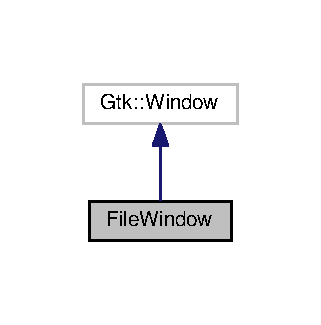
\includegraphics[width=154pt]{class_file_window__inherit__graph}
\end{center}
\end{figure}


Collaboration diagram for File\+Window\+:
\nopagebreak
\begin{figure}[H]
\begin{center}
\leavevmode
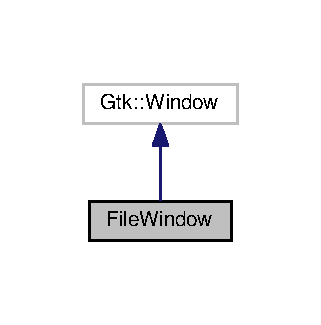
\includegraphics[width=154pt]{class_file_window__coll__graph}
\end{center}
\end{figure}
\subsection*{Public Member Functions}
\begin{DoxyCompactItemize}
\item 
\hyperlink{class_file_window_aa90776803aafb4745b145620e7f8390a}{File\+Window} ()
\item 
virtual \hyperlink{class_file_window_aa699c56901fb51fbc3a6646f999d83f1}{$\sim$\+File\+Window} ()
\end{DoxyCompactItemize}
\subsection*{Protected Member Functions}
\begin{DoxyCompactItemize}
\item 
void \hyperlink{class_file_window_a5bee1d5abb06d758c34836ae03536a5b}{on\+\_\+button\+\_\+file\+\_\+clicked} ()
\end{DoxyCompactItemize}
\subsection*{Protected Attributes}
\begin{DoxyCompactItemize}
\item 
Gtk\+::\+Button\+Box \hyperlink{class_file_window_afa6c56d7516fb2a8cbee798ef298b646}{m\+\_\+\+Button\+Box}
\item 
Gtk\+::\+Button \hyperlink{class_file_window_acf6526bcbac19ea8e0295b3601f78f05}{m\+\_\+\+Button\+\_\+\+File}
\end{DoxyCompactItemize}


\subsection{Constructor \& Destructor Documentation}
\index{File\+Window@{File\+Window}!File\+Window@{File\+Window}}
\index{File\+Window@{File\+Window}!File\+Window@{File\+Window}}
\subsubsection[{\texorpdfstring{File\+Window()}{FileWindow()}}]{\setlength{\rightskip}{0pt plus 5cm}File\+Window\+::\+File\+Window (
\begin{DoxyParamCaption}
{}
\end{DoxyParamCaption}
)}\hypertarget{class_file_window_aa90776803aafb4745b145620e7f8390a}{}\label{class_file_window_aa90776803aafb4745b145620e7f8390a}


Here is the call graph for this function\+:
\nopagebreak
\begin{figure}[H]
\begin{center}
\leavevmode
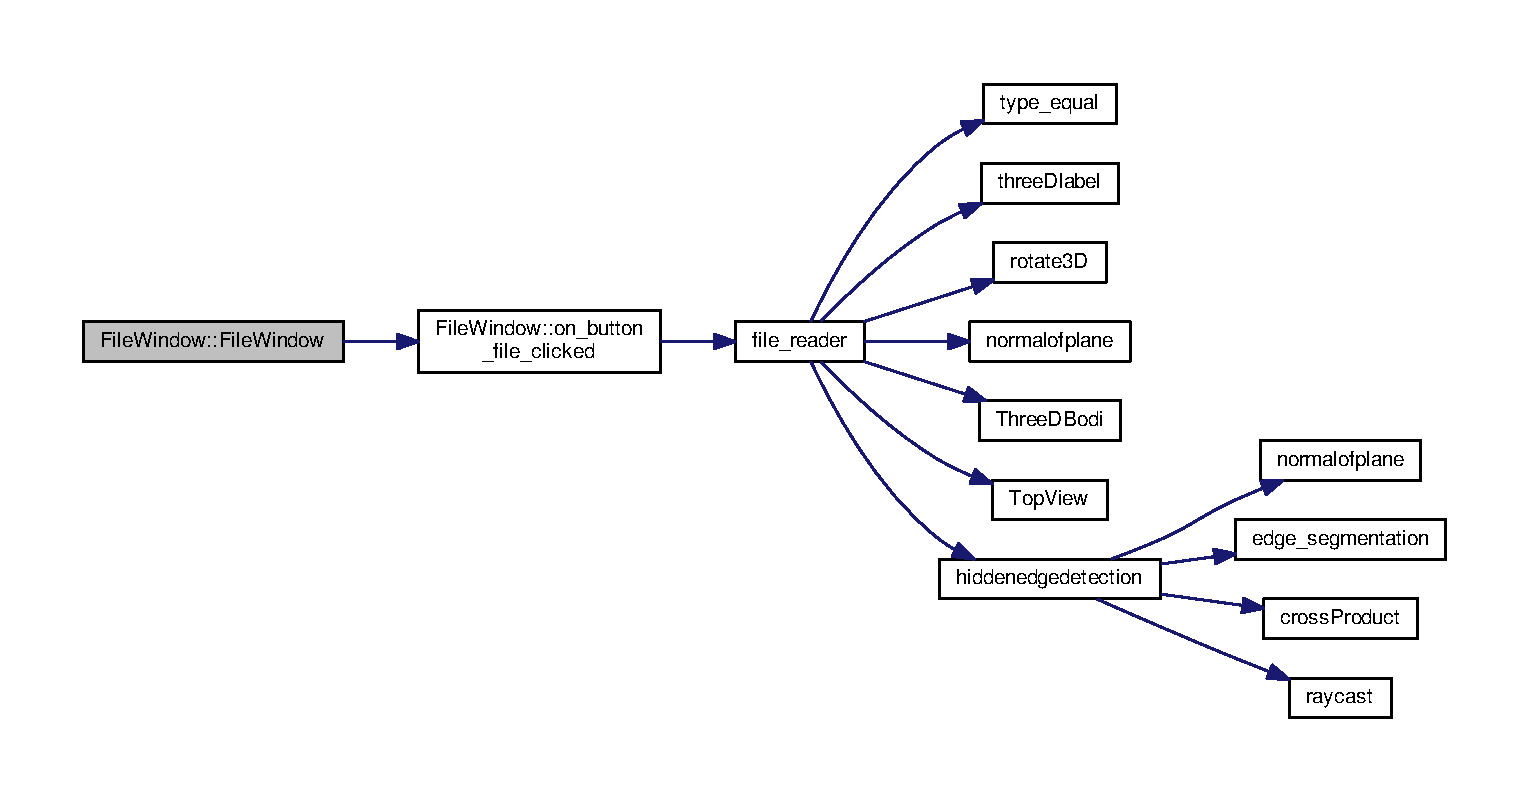
\includegraphics[width=350pt]{class_file_window_aa90776803aafb4745b145620e7f8390a_cgraph}
\end{center}
\end{figure}


\index{File\+Window@{File\+Window}!````~File\+Window@{$\sim$\+File\+Window}}
\index{````~File\+Window@{$\sim$\+File\+Window}!File\+Window@{File\+Window}}
\subsubsection[{\texorpdfstring{$\sim$\+File\+Window()}{~FileWindow()}}]{\setlength{\rightskip}{0pt plus 5cm}File\+Window\+::$\sim$\+File\+Window (
\begin{DoxyParamCaption}
{}
\end{DoxyParamCaption}
)\hspace{0.3cm}{\ttfamily [virtual]}}\hypertarget{class_file_window_aa699c56901fb51fbc3a6646f999d83f1}{}\label{class_file_window_aa699c56901fb51fbc3a6646f999d83f1}


\subsection{Member Function Documentation}
\index{File\+Window@{File\+Window}!on\+\_\+button\+\_\+file\+\_\+clicked@{on\+\_\+button\+\_\+file\+\_\+clicked}}
\index{on\+\_\+button\+\_\+file\+\_\+clicked@{on\+\_\+button\+\_\+file\+\_\+clicked}!File\+Window@{File\+Window}}
\subsubsection[{\texorpdfstring{on\+\_\+button\+\_\+file\+\_\+clicked()}{on_button_file_clicked()}}]{\setlength{\rightskip}{0pt plus 5cm}void File\+Window\+::on\+\_\+button\+\_\+file\+\_\+clicked (
\begin{DoxyParamCaption}
{}
\end{DoxyParamCaption}
)\hspace{0.3cm}{\ttfamily [protected]}}\hypertarget{class_file_window_a5bee1d5abb06d758c34836ae03536a5b}{}\label{class_file_window_a5bee1d5abb06d758c34836ae03536a5b}


Here is the call graph for this function\+:
\nopagebreak
\begin{figure}[H]
\begin{center}
\leavevmode
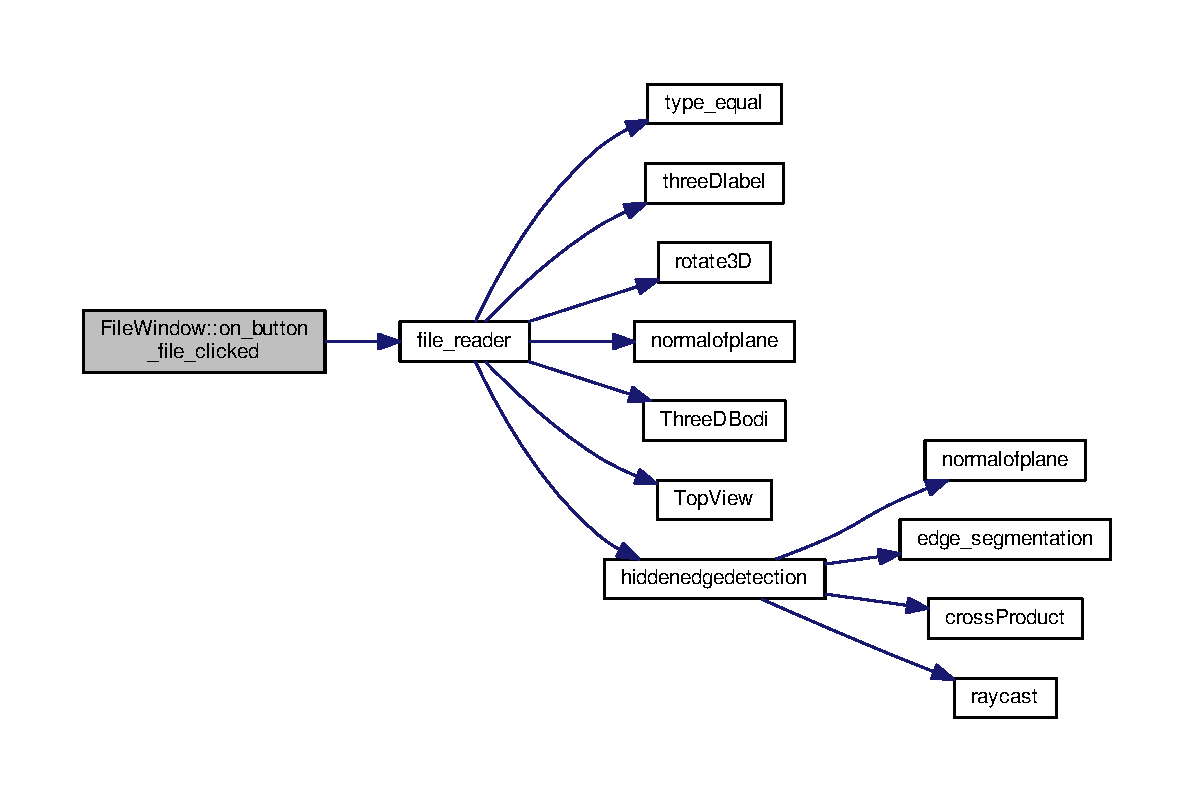
\includegraphics[width=350pt]{class_file_window_a5bee1d5abb06d758c34836ae03536a5b_cgraph}
\end{center}
\end{figure}




\subsection{Member Data Documentation}
\index{File\+Window@{File\+Window}!m\+\_\+\+Button\+\_\+\+File@{m\+\_\+\+Button\+\_\+\+File}}
\index{m\+\_\+\+Button\+\_\+\+File@{m\+\_\+\+Button\+\_\+\+File}!File\+Window@{File\+Window}}
\subsubsection[{\texorpdfstring{m\+\_\+\+Button\+\_\+\+File}{m_Button_File}}]{\setlength{\rightskip}{0pt plus 5cm}Gtk\+::\+Button File\+Window\+::m\+\_\+\+Button\+\_\+\+File\hspace{0.3cm}{\ttfamily [protected]}}\hypertarget{class_file_window_acf6526bcbac19ea8e0295b3601f78f05}{}\label{class_file_window_acf6526bcbac19ea8e0295b3601f78f05}
\index{File\+Window@{File\+Window}!m\+\_\+\+Button\+Box@{m\+\_\+\+Button\+Box}}
\index{m\+\_\+\+Button\+Box@{m\+\_\+\+Button\+Box}!File\+Window@{File\+Window}}
\subsubsection[{\texorpdfstring{m\+\_\+\+Button\+Box}{m_ButtonBox}}]{\setlength{\rightskip}{0pt plus 5cm}Gtk\+::\+Button\+Box File\+Window\+::m\+\_\+\+Button\+Box\hspace{0.3cm}{\ttfamily [protected]}}\hypertarget{class_file_window_afa6c56d7516fb2a8cbee798ef298b646}{}\label{class_file_window_afa6c56d7516fb2a8cbee798ef298b646}


The documentation for this class was generated from the following files\+:\begin{DoxyCompactItemize}
\item 
C\+O\+P290new/include/\hyperlink{myarea_8h}{myarea.\+h}\item 
C\+O\+P290new/src/\hyperlink{_main_8cpp}{Main.\+cpp}\end{DoxyCompactItemize}

\hypertarget{class_hidden_edge}{}\section{Hidden\+Edge Class Reference}
\label{class_hidden_edge}\index{Hidden\+Edge@{Hidden\+Edge}}


{\ttfamily \#include $<$2\+D.\+h$>$}

\subsection*{Public Member Functions}
\begin{DoxyCompactItemize}
\item 
void \hyperlink{class_hidden_edge_a95880769d5769f2928619ac0e059d12b}{translatex} (float dx)
\item 
void \hyperlink{class_hidden_edge_a123831d74de8e55ddb36212f1b518617}{translatey} (float dy)
\item 
void \hyperlink{class_hidden_edge_ab4196074b4b4a67077b278a4a984c3cc}{rotate} (float delta, bool dirdelta, \hyperlink{class_vertex2_d}{Vertex2D} axis)
\end{DoxyCompactItemize}
\subsection*{Public Attributes}
\begin{DoxyCompactItemize}
\item 
float \hyperlink{class_hidden_edge_a2370e1eea3d938266390f56b95dae210}{x1}
\item 
float \hyperlink{class_hidden_edge_a7e1436e8b31eca0d8b944d81ff9238a1}{y1}
\item 
float \hyperlink{class_hidden_edge_a72b1bbd570ebb6f6e0c473d0aebd9c0a}{x2}
\item 
float \hyperlink{class_hidden_edge_a63af4b7204c511284e364a8fede55d46}{y2}
\end{DoxyCompactItemize}


\subsection{Member Function Documentation}
\index{Hidden\+Edge@{Hidden\+Edge}!rotate@{rotate}}
\index{rotate@{rotate}!Hidden\+Edge@{Hidden\+Edge}}
\subsubsection[{\texorpdfstring{rotate(float delta, bool dirdelta, Vertex2\+D axis)}{rotate(float delta, bool dirdelta, Vertex2D axis)}}]{\setlength{\rightskip}{0pt plus 5cm}void Hidden\+Edge\+::rotate (
\begin{DoxyParamCaption}
\item[{float}]{delta, }
\item[{bool}]{dirdelta, }
\item[{{\bf Vertex2D}}]{axis}
\end{DoxyParamCaption}
)\hspace{0.3cm}{\ttfamily [inline]}}\hypertarget{class_hidden_edge_ab4196074b4b4a67077b278a4a984c3cc}{}\label{class_hidden_edge_ab4196074b4b4a67077b278a4a984c3cc}
\index{Hidden\+Edge@{Hidden\+Edge}!translatex@{translatex}}
\index{translatex@{translatex}!Hidden\+Edge@{Hidden\+Edge}}
\subsubsection[{\texorpdfstring{translatex(float dx)}{translatex(float dx)}}]{\setlength{\rightskip}{0pt plus 5cm}void Hidden\+Edge\+::translatex (
\begin{DoxyParamCaption}
\item[{float}]{dx}
\end{DoxyParamCaption}
)\hspace{0.3cm}{\ttfamily [inline]}}\hypertarget{class_hidden_edge_a95880769d5769f2928619ac0e059d12b}{}\label{class_hidden_edge_a95880769d5769f2928619ac0e059d12b}
\index{Hidden\+Edge@{Hidden\+Edge}!translatey@{translatey}}
\index{translatey@{translatey}!Hidden\+Edge@{Hidden\+Edge}}
\subsubsection[{\texorpdfstring{translatey(float dy)}{translatey(float dy)}}]{\setlength{\rightskip}{0pt plus 5cm}void Hidden\+Edge\+::translatey (
\begin{DoxyParamCaption}
\item[{float}]{dy}
\end{DoxyParamCaption}
)\hspace{0.3cm}{\ttfamily [inline]}}\hypertarget{class_hidden_edge_a123831d74de8e55ddb36212f1b518617}{}\label{class_hidden_edge_a123831d74de8e55ddb36212f1b518617}


\subsection{Member Data Documentation}
\index{Hidden\+Edge@{Hidden\+Edge}!x1@{x1}}
\index{x1@{x1}!Hidden\+Edge@{Hidden\+Edge}}
\subsubsection[{\texorpdfstring{x1}{x1}}]{\setlength{\rightskip}{0pt plus 5cm}float Hidden\+Edge\+::x1}\hypertarget{class_hidden_edge_a2370e1eea3d938266390f56b95dae210}{}\label{class_hidden_edge_a2370e1eea3d938266390f56b95dae210}
\index{Hidden\+Edge@{Hidden\+Edge}!x2@{x2}}
\index{x2@{x2}!Hidden\+Edge@{Hidden\+Edge}}
\subsubsection[{\texorpdfstring{x2}{x2}}]{\setlength{\rightskip}{0pt plus 5cm}float Hidden\+Edge\+::x2}\hypertarget{class_hidden_edge_a72b1bbd570ebb6f6e0c473d0aebd9c0a}{}\label{class_hidden_edge_a72b1bbd570ebb6f6e0c473d0aebd9c0a}
\index{Hidden\+Edge@{Hidden\+Edge}!y1@{y1}}
\index{y1@{y1}!Hidden\+Edge@{Hidden\+Edge}}
\subsubsection[{\texorpdfstring{y1}{y1}}]{\setlength{\rightskip}{0pt plus 5cm}float Hidden\+Edge\+::y1}\hypertarget{class_hidden_edge_a7e1436e8b31eca0d8b944d81ff9238a1}{}\label{class_hidden_edge_a7e1436e8b31eca0d8b944d81ff9238a1}
\index{Hidden\+Edge@{Hidden\+Edge}!y2@{y2}}
\index{y2@{y2}!Hidden\+Edge@{Hidden\+Edge}}
\subsubsection[{\texorpdfstring{y2}{y2}}]{\setlength{\rightskip}{0pt plus 5cm}float Hidden\+Edge\+::y2}\hypertarget{class_hidden_edge_a63af4b7204c511284e364a8fede55d46}{}\label{class_hidden_edge_a63af4b7204c511284e364a8fede55d46}


The documentation for this class was generated from the following file\+:\begin{DoxyCompactItemize}
\item 
/home/hp/\+Desktop/\+C\+O\+P290/\hyperlink{2_d_8h}{2\+D.\+h}\end{DoxyCompactItemize}

\hypertarget{class_hidden_edge3_d}{}\section{Hidden\+Edge3D Class Reference}
\label{class_hidden_edge3_d}\index{Hidden\+Edge3D@{Hidden\+Edge3D}}


{\ttfamily \#include $<$3\+D.\+h$>$}

\subsection*{Public Member Functions}
\begin{DoxyCompactItemize}
\item 
void \hyperlink{class_hidden_edge3_d_af52b93b4ec291277aaf5c1138068f6db}{rotatex} (double delta, bool dirdelta)
\item 
void \hyperlink{class_hidden_edge3_d_aacf1c6981dc9189b56de6f0920e146ce}{rotatey} (double delta, bool dirdelta)
\item 
void \hyperlink{class_hidden_edge3_d_acf087a769831355854758b043e9b4bfa}{rotatez} (double delta, bool dirdelta)
\item 
void \hyperlink{class_hidden_edge3_d_a47c13f15de3ae05d2ea539ed094084e9}{rotate} (double deltax, bool dirx, double deltay, bool diry, double deltaz, bool dirz)
\end{DoxyCompactItemize}
\subsection*{Public Attributes}
\begin{DoxyCompactItemize}
\item 
double \hyperlink{class_hidden_edge3_d_a2427c2c64f2923c487e4a05623ba58bb}{x1}
\item 
double \hyperlink{class_hidden_edge3_d_a40b67744e7d07d47204599c5481f5d2e}{y1}
\item 
double \hyperlink{class_hidden_edge3_d_ad8b9d5b2867873171153447a1f75204e}{z1}
\item 
double \hyperlink{class_hidden_edge3_d_adeba8473617de2da7c6276b8f7806fa0}{x2}
\item 
double \hyperlink{class_hidden_edge3_d_ab8a6f5b37b5b208042307a8a1060bd0d}{y2}
\item 
double \hyperlink{class_hidden_edge3_d_a6e4a7847916c1849577b18d5823c5e50}{z2}
\end{DoxyCompactItemize}


\subsection{Member Function Documentation}
\index{Hidden\+Edge3D@{Hidden\+Edge3D}!rotate@{rotate}}
\index{rotate@{rotate}!Hidden\+Edge3D@{Hidden\+Edge3D}}
\subsubsection[{\texorpdfstring{rotate(double deltax, bool dirx, double deltay, bool diry, double deltaz, bool dirz)}{rotate(double deltax, bool dirx, double deltay, bool diry, double deltaz, bool dirz)}}]{\setlength{\rightskip}{0pt plus 5cm}void Hidden\+Edge3\+D\+::rotate (
\begin{DoxyParamCaption}
\item[{double}]{deltax, }
\item[{bool}]{dirx, }
\item[{double}]{deltay, }
\item[{bool}]{diry, }
\item[{double}]{deltaz, }
\item[{bool}]{dirz}
\end{DoxyParamCaption}
)}\hypertarget{class_hidden_edge3_d_a47c13f15de3ae05d2ea539ed094084e9}{}\label{class_hidden_edge3_d_a47c13f15de3ae05d2ea539ed094084e9}


Here is the call graph for this function\+:
\nopagebreak
\begin{figure}[H]
\begin{center}
\leavevmode
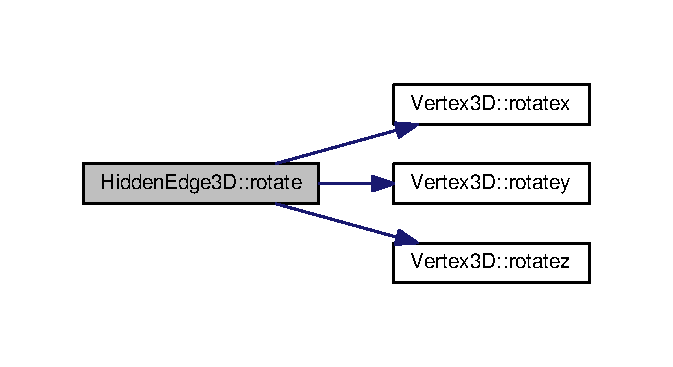
\includegraphics[width=323pt]{class_hidden_edge3_d_a47c13f15de3ae05d2ea539ed094084e9_cgraph}
\end{center}
\end{figure}


\index{Hidden\+Edge3D@{Hidden\+Edge3D}!rotatex@{rotatex}}
\index{rotatex@{rotatex}!Hidden\+Edge3D@{Hidden\+Edge3D}}
\subsubsection[{\texorpdfstring{rotatex(double delta, bool dirdelta)}{rotatex(double delta, bool dirdelta)}}]{\setlength{\rightskip}{0pt plus 5cm}void Hidden\+Edge3\+D\+::rotatex (
\begin{DoxyParamCaption}
\item[{double}]{delta, }
\item[{bool}]{dirdelta}
\end{DoxyParamCaption}
)}\hypertarget{class_hidden_edge3_d_af52b93b4ec291277aaf5c1138068f6db}{}\label{class_hidden_edge3_d_af52b93b4ec291277aaf5c1138068f6db}
\index{Hidden\+Edge3D@{Hidden\+Edge3D}!rotatey@{rotatey}}
\index{rotatey@{rotatey}!Hidden\+Edge3D@{Hidden\+Edge3D}}
\subsubsection[{\texorpdfstring{rotatey(double delta, bool dirdelta)}{rotatey(double delta, bool dirdelta)}}]{\setlength{\rightskip}{0pt plus 5cm}void Hidden\+Edge3\+D\+::rotatey (
\begin{DoxyParamCaption}
\item[{double}]{delta, }
\item[{bool}]{dirdelta}
\end{DoxyParamCaption}
)}\hypertarget{class_hidden_edge3_d_aacf1c6981dc9189b56de6f0920e146ce}{}\label{class_hidden_edge3_d_aacf1c6981dc9189b56de6f0920e146ce}
\index{Hidden\+Edge3D@{Hidden\+Edge3D}!rotatez@{rotatez}}
\index{rotatez@{rotatez}!Hidden\+Edge3D@{Hidden\+Edge3D}}
\subsubsection[{\texorpdfstring{rotatez(double delta, bool dirdelta)}{rotatez(double delta, bool dirdelta)}}]{\setlength{\rightskip}{0pt plus 5cm}void Hidden\+Edge3\+D\+::rotatez (
\begin{DoxyParamCaption}
\item[{double}]{delta, }
\item[{bool}]{dirdelta}
\end{DoxyParamCaption}
)}\hypertarget{class_hidden_edge3_d_acf087a769831355854758b043e9b4bfa}{}\label{class_hidden_edge3_d_acf087a769831355854758b043e9b4bfa}


\subsection{Member Data Documentation}
\index{Hidden\+Edge3D@{Hidden\+Edge3D}!x1@{x1}}
\index{x1@{x1}!Hidden\+Edge3D@{Hidden\+Edge3D}}
\subsubsection[{\texorpdfstring{x1}{x1}}]{\setlength{\rightskip}{0pt plus 5cm}double Hidden\+Edge3\+D\+::x1}\hypertarget{class_hidden_edge3_d_a2427c2c64f2923c487e4a05623ba58bb}{}\label{class_hidden_edge3_d_a2427c2c64f2923c487e4a05623ba58bb}
\index{Hidden\+Edge3D@{Hidden\+Edge3D}!x2@{x2}}
\index{x2@{x2}!Hidden\+Edge3D@{Hidden\+Edge3D}}
\subsubsection[{\texorpdfstring{x2}{x2}}]{\setlength{\rightskip}{0pt plus 5cm}double Hidden\+Edge3\+D\+::x2}\hypertarget{class_hidden_edge3_d_adeba8473617de2da7c6276b8f7806fa0}{}\label{class_hidden_edge3_d_adeba8473617de2da7c6276b8f7806fa0}
\index{Hidden\+Edge3D@{Hidden\+Edge3D}!y1@{y1}}
\index{y1@{y1}!Hidden\+Edge3D@{Hidden\+Edge3D}}
\subsubsection[{\texorpdfstring{y1}{y1}}]{\setlength{\rightskip}{0pt plus 5cm}double Hidden\+Edge3\+D\+::y1}\hypertarget{class_hidden_edge3_d_a40b67744e7d07d47204599c5481f5d2e}{}\label{class_hidden_edge3_d_a40b67744e7d07d47204599c5481f5d2e}
\index{Hidden\+Edge3D@{Hidden\+Edge3D}!y2@{y2}}
\index{y2@{y2}!Hidden\+Edge3D@{Hidden\+Edge3D}}
\subsubsection[{\texorpdfstring{y2}{y2}}]{\setlength{\rightskip}{0pt plus 5cm}double Hidden\+Edge3\+D\+::y2}\hypertarget{class_hidden_edge3_d_ab8a6f5b37b5b208042307a8a1060bd0d}{}\label{class_hidden_edge3_d_ab8a6f5b37b5b208042307a8a1060bd0d}
\index{Hidden\+Edge3D@{Hidden\+Edge3D}!z1@{z1}}
\index{z1@{z1}!Hidden\+Edge3D@{Hidden\+Edge3D}}
\subsubsection[{\texorpdfstring{z1}{z1}}]{\setlength{\rightskip}{0pt plus 5cm}double Hidden\+Edge3\+D\+::z1}\hypertarget{class_hidden_edge3_d_ad8b9d5b2867873171153447a1f75204e}{}\label{class_hidden_edge3_d_ad8b9d5b2867873171153447a1f75204e}
\index{Hidden\+Edge3D@{Hidden\+Edge3D}!z2@{z2}}
\index{z2@{z2}!Hidden\+Edge3D@{Hidden\+Edge3D}}
\subsubsection[{\texorpdfstring{z2}{z2}}]{\setlength{\rightskip}{0pt plus 5cm}double Hidden\+Edge3\+D\+::z2}\hypertarget{class_hidden_edge3_d_a6e4a7847916c1849577b18d5823c5e50}{}\label{class_hidden_edge3_d_a6e4a7847916c1849577b18d5823c5e50}


The documentation for this class was generated from the following files\+:\begin{DoxyCompactItemize}
\item 
C\+O\+P290new/include/\hyperlink{3_d_8h}{3\+D.\+h}\item 
C\+O\+P290new/src/\hyperlink{3_d_8cpp}{3\+D.\+cpp}\end{DoxyCompactItemize}

\hypertarget{class_label}{}\section{Label Class Reference}
\label{class_label}\index{Label@{Label}}


{\ttfamily \#include $<$2\+D.\+h$>$}

\subsection*{Public Attributes}
\begin{DoxyCompactItemize}
\item 
string \hyperlink{class_label_a8521f1088bbc065c997a428afed1ed3e}{label}
\end{DoxyCompactItemize}


\subsection{Member Data Documentation}
\index{Label@{Label}!label@{label}}
\index{label@{label}!Label@{Label}}
\subsubsection[{\texorpdfstring{label}{label}}]{\setlength{\rightskip}{0pt plus 5cm}string Label\+::label}\hypertarget{class_label_a8521f1088bbc065c997a428afed1ed3e}{}\label{class_label_a8521f1088bbc065c997a428afed1ed3e}


The documentation for this class was generated from the following file\+:\begin{DoxyCompactItemize}
\item 
C\+O\+P290new/include/\hyperlink{2_d_8h}{2\+D.\+h}\end{DoxyCompactItemize}

\hypertarget{class_labelled2_d}{}\section{Labelled2D Class Reference}
\label{class_labelled2_d}\index{Labelled2D@{Labelled2D}}


{\ttfamily \#include $<$2\+D.\+h$>$}

\subsection*{Public Attributes}
\begin{DoxyCompactItemize}
\item 
std\+::vector$<$ \hyperlink{class_vertex2_d}{Vertex2D} $>$ \hyperlink{class_labelled2_d_ab677e79d5e4bcfebbeb83dc38e5511e4}{v}
\item 
std\+::vector$<$ \hyperlink{class_visible_edge}{Visible\+Edge} $>$ \hyperlink{class_labelled2_d_ade711f960ea78222660c68b7ea29840b}{ve}
\item 
std\+::vector$<$ \hyperlink{class_hidden_edge}{Hidden\+Edge} $>$ \hyperlink{class_labelled2_d_a166043f03faf313ef3772c14daf2604f}{he}
\item 
std\+::vector$<$ \hyperlink{class_label}{Label} $>$ \hyperlink{class_labelled2_d_a16b9a518c00306b5183d1775339efeff}{lbl}
\end{DoxyCompactItemize}


\subsection{Member Data Documentation}
\index{Labelled2D@{Labelled2D}!he@{he}}
\index{he@{he}!Labelled2D@{Labelled2D}}
\subsubsection[{\texorpdfstring{he}{he}}]{\setlength{\rightskip}{0pt plus 5cm}std\+::vector$<${\bf Hidden\+Edge}$>$ Labelled2\+D\+::he}\hypertarget{class_labelled2_d_a166043f03faf313ef3772c14daf2604f}{}\label{class_labelled2_d_a166043f03faf313ef3772c14daf2604f}
\index{Labelled2D@{Labelled2D}!lbl@{lbl}}
\index{lbl@{lbl}!Labelled2D@{Labelled2D}}
\subsubsection[{\texorpdfstring{lbl}{lbl}}]{\setlength{\rightskip}{0pt plus 5cm}std\+::vector$<${\bf Label}$>$ Labelled2\+D\+::lbl}\hypertarget{class_labelled2_d_a16b9a518c00306b5183d1775339efeff}{}\label{class_labelled2_d_a16b9a518c00306b5183d1775339efeff}
\index{Labelled2D@{Labelled2D}!v@{v}}
\index{v@{v}!Labelled2D@{Labelled2D}}
\subsubsection[{\texorpdfstring{v}{v}}]{\setlength{\rightskip}{0pt plus 5cm}std\+::vector$<${\bf Vertex2D}$>$ Labelled2\+D\+::v}\hypertarget{class_labelled2_d_ab677e79d5e4bcfebbeb83dc38e5511e4}{}\label{class_labelled2_d_ab677e79d5e4bcfebbeb83dc38e5511e4}
\index{Labelled2D@{Labelled2D}!ve@{ve}}
\index{ve@{ve}!Labelled2D@{Labelled2D}}
\subsubsection[{\texorpdfstring{ve}{ve}}]{\setlength{\rightskip}{0pt plus 5cm}std\+::vector$<${\bf Visible\+Edge}$>$ Labelled2\+D\+::ve}\hypertarget{class_labelled2_d_ade711f960ea78222660c68b7ea29840b}{}\label{class_labelled2_d_ade711f960ea78222660c68b7ea29840b}


The documentation for this class was generated from the following file\+:\begin{DoxyCompactItemize}
\item 
C\+O\+P290new/include/\hyperlink{2_d_8h}{2\+D.\+h}\end{DoxyCompactItemize}

\hypertarget{class_my_window}{}\section{My\+Window Class Reference}
\label{class_my_window}\index{My\+Window@{My\+Window}}


{\ttfamily \#include $<$myarea.\+h$>$}



Inheritance diagram for My\+Window\+:
\nopagebreak
\begin{figure}[H]
\begin{center}
\leavevmode
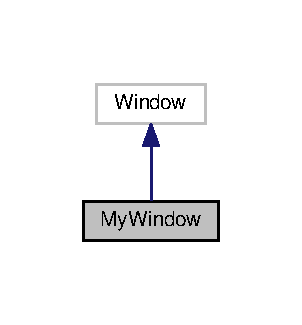
\includegraphics[width=145pt]{class_my_window__inherit__graph}
\end{center}
\end{figure}


Collaboration diagram for My\+Window\+:
\nopagebreak
\begin{figure}[H]
\begin{center}
\leavevmode
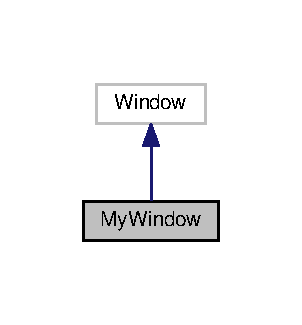
\includegraphics[width=145pt]{class_my_window__coll__graph}
\end{center}
\end{figure}
\subsection*{Public Member Functions}
\begin{DoxyCompactItemize}
\item 
\hyperlink{class_my_window_ae0ae4de3a21d55202f428bd6bf5656d9}{My\+Window} ()
\item 
virtual \hyperlink{class_my_window_acc6b33f79cb9f1ee9107beac4c474fd3}{$\sim$\+My\+Window} ()
\end{DoxyCompactItemize}
\subsection*{Protected Member Functions}
\begin{DoxyCompactItemize}
\item 
bool \hyperlink{class_my_window_aa800cd5778892613b4355b016041cc23}{on\+\_\+drawe} (const Cairo\+::\+Ref\+Ptr$<$ Cairo\+::\+Context $>$ \&cr)
\item 
void \hyperlink{class_my_window_af11dea8ab3785a9e473ebc70518d61ed}{on\+\_\+click} (int x)
\end{DoxyCompactItemize}
\subsection*{Protected Attributes}
\begin{DoxyCompactItemize}
\item 
Gtk\+::\+Grid \hyperlink{class_my_window_a1bd2ae9ce185432e826e238b61151af1}{grid}
\item 
Gtk\+::\+Drawing\+Area \hyperlink{class_my_window_aa98997a3b779b010640c90a1fd094bf9}{area}
\item 
Gtk\+::\+Button \hyperlink{class_my_window_aeeaad7113b758654a926a50229339910}{buttonx}
\item 
Gtk\+::\+Button \hyperlink{class_my_window_abf7f5f0ba789dd4a23893169a0ef100c}{buttony}
\item 
Gtk\+::\+Button \hyperlink{class_my_window_a5b82afccc869f5bd51d0482633684b60}{buttonz}
\end{DoxyCompactItemize}


\subsection{Constructor \& Destructor Documentation}
\index{My\+Window@{My\+Window}!My\+Window@{My\+Window}}
\index{My\+Window@{My\+Window}!My\+Window@{My\+Window}}
\subsubsection[{\texorpdfstring{My\+Window()}{MyWindow()}}]{\setlength{\rightskip}{0pt plus 5cm}My\+Window\+::\+My\+Window (
\begin{DoxyParamCaption}
{}
\end{DoxyParamCaption}
)}\hypertarget{class_my_window_ae0ae4de3a21d55202f428bd6bf5656d9}{}\label{class_my_window_ae0ae4de3a21d55202f428bd6bf5656d9}


Here is the call graph for this function\+:
\nopagebreak
\begin{figure}[H]
\begin{center}
\leavevmode
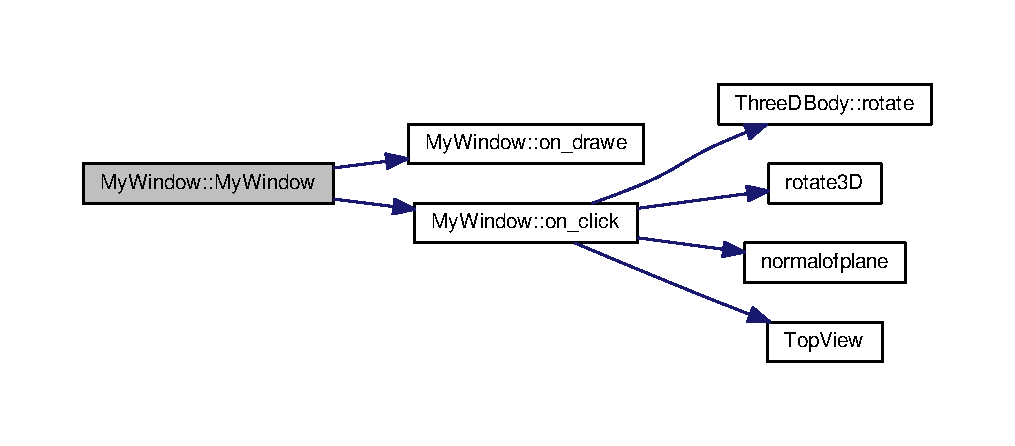
\includegraphics[width=350pt]{class_my_window_ae0ae4de3a21d55202f428bd6bf5656d9_cgraph}
\end{center}
\end{figure}


\index{My\+Window@{My\+Window}!````~My\+Window@{$\sim$\+My\+Window}}
\index{````~My\+Window@{$\sim$\+My\+Window}!My\+Window@{My\+Window}}
\subsubsection[{\texorpdfstring{$\sim$\+My\+Window()}{~MyWindow()}}]{\setlength{\rightskip}{0pt plus 5cm}My\+Window\+::$\sim$\+My\+Window (
\begin{DoxyParamCaption}
{}
\end{DoxyParamCaption}
)\hspace{0.3cm}{\ttfamily [virtual]}}\hypertarget{class_my_window_acc6b33f79cb9f1ee9107beac4c474fd3}{}\label{class_my_window_acc6b33f79cb9f1ee9107beac4c474fd3}


\subsection{Member Function Documentation}
\index{My\+Window@{My\+Window}!on\+\_\+click@{on\+\_\+click}}
\index{on\+\_\+click@{on\+\_\+click}!My\+Window@{My\+Window}}
\subsubsection[{\texorpdfstring{on\+\_\+click(int x)}{on_click(int x)}}]{\setlength{\rightskip}{0pt plus 5cm}void My\+Window\+::on\+\_\+click (
\begin{DoxyParamCaption}
\item[{int}]{x}
\end{DoxyParamCaption}
)\hspace{0.3cm}{\ttfamily [protected]}}\hypertarget{class_my_window_af11dea8ab3785a9e473ebc70518d61ed}{}\label{class_my_window_af11dea8ab3785a9e473ebc70518d61ed}


Here is the call graph for this function\+:
\nopagebreak
\begin{figure}[H]
\begin{center}
\leavevmode
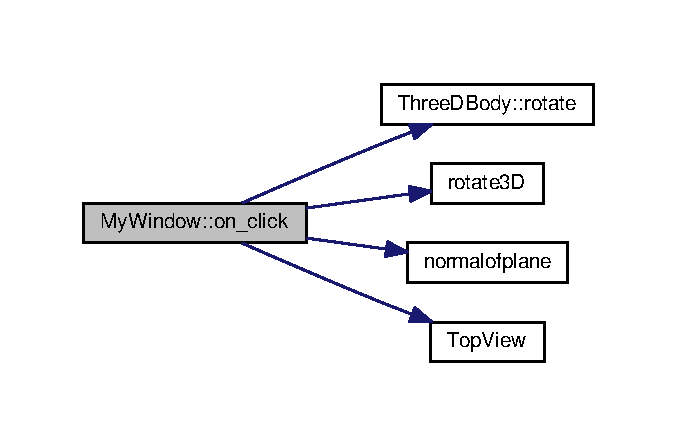
\includegraphics[width=325pt]{class_my_window_af11dea8ab3785a9e473ebc70518d61ed_cgraph}
\end{center}
\end{figure}


\index{My\+Window@{My\+Window}!on\+\_\+drawe@{on\+\_\+drawe}}
\index{on\+\_\+drawe@{on\+\_\+drawe}!My\+Window@{My\+Window}}
\subsubsection[{\texorpdfstring{on\+\_\+drawe(const Cairo\+::\+Ref\+Ptr$<$ Cairo\+::\+Context $>$ \&cr)}{on_drawe(const Cairo::RefPtr< Cairo::Context > &cr)}}]{\setlength{\rightskip}{0pt plus 5cm}bool My\+Window\+::on\+\_\+drawe (
\begin{DoxyParamCaption}
\item[{const Cairo\+::\+Ref\+Ptr$<$ Cairo\+::\+Context $>$ \&}]{cr}
\end{DoxyParamCaption}
)\hspace{0.3cm}{\ttfamily [protected]}}\hypertarget{class_my_window_aa800cd5778892613b4355b016041cc23}{}\label{class_my_window_aa800cd5778892613b4355b016041cc23}


\subsection{Member Data Documentation}
\index{My\+Window@{My\+Window}!area@{area}}
\index{area@{area}!My\+Window@{My\+Window}}
\subsubsection[{\texorpdfstring{area}{area}}]{\setlength{\rightskip}{0pt plus 5cm}Gtk\+::\+Drawing\+Area My\+Window\+::area\hspace{0.3cm}{\ttfamily [protected]}}\hypertarget{class_my_window_aa98997a3b779b010640c90a1fd094bf9}{}\label{class_my_window_aa98997a3b779b010640c90a1fd094bf9}
\index{My\+Window@{My\+Window}!buttonx@{buttonx}}
\index{buttonx@{buttonx}!My\+Window@{My\+Window}}
\subsubsection[{\texorpdfstring{buttonx}{buttonx}}]{\setlength{\rightskip}{0pt plus 5cm}Gtk\+::\+Button My\+Window\+::buttonx\hspace{0.3cm}{\ttfamily [protected]}}\hypertarget{class_my_window_aeeaad7113b758654a926a50229339910}{}\label{class_my_window_aeeaad7113b758654a926a50229339910}
\index{My\+Window@{My\+Window}!buttony@{buttony}}
\index{buttony@{buttony}!My\+Window@{My\+Window}}
\subsubsection[{\texorpdfstring{buttony}{buttony}}]{\setlength{\rightskip}{0pt plus 5cm}Gtk\+::\+Button My\+Window\+::buttony\hspace{0.3cm}{\ttfamily [protected]}}\hypertarget{class_my_window_abf7f5f0ba789dd4a23893169a0ef100c}{}\label{class_my_window_abf7f5f0ba789dd4a23893169a0ef100c}
\index{My\+Window@{My\+Window}!buttonz@{buttonz}}
\index{buttonz@{buttonz}!My\+Window@{My\+Window}}
\subsubsection[{\texorpdfstring{buttonz}{buttonz}}]{\setlength{\rightskip}{0pt plus 5cm}Gtk\+::\+Button My\+Window\+::buttonz\hspace{0.3cm}{\ttfamily [protected]}}\hypertarget{class_my_window_a5b82afccc869f5bd51d0482633684b60}{}\label{class_my_window_a5b82afccc869f5bd51d0482633684b60}
\index{My\+Window@{My\+Window}!grid@{grid}}
\index{grid@{grid}!My\+Window@{My\+Window}}
\subsubsection[{\texorpdfstring{grid}{grid}}]{\setlength{\rightskip}{0pt plus 5cm}Gtk\+::\+Grid My\+Window\+::grid\hspace{0.3cm}{\ttfamily [protected]}}\hypertarget{class_my_window_a1bd2ae9ce185432e826e238b61151af1}{}\label{class_my_window_a1bd2ae9ce185432e826e238b61151af1}


The documentation for this class was generated from the following files\+:\begin{DoxyCompactItemize}
\item 
C\+O\+P290new/include/\hyperlink{myarea_8h}{myarea.\+h}\item 
C\+O\+P290new/src/\hyperlink{3_dto2_d_8cpp}{3\+Dto2\+D.\+cpp}\end{DoxyCompactItemize}

\hypertarget{class_orthographic_view}{}\section{Orthographic\+View Class Reference}
\label{class_orthographic_view}\index{Orthographic\+View@{Orthographic\+View}}


{\ttfamily \#include $<$2\+D.\+h$>$}

\subsection*{Public Attributes}
\begin{DoxyCompactItemize}
\item 
int \hyperlink{class_orthographic_view_ae9f5b34d51d46495fd507dfa8f0c352b}{view\+\_\+type}
\end{DoxyCompactItemize}


\subsection{Member Data Documentation}
\index{Orthographic\+View@{Orthographic\+View}!view\+\_\+type@{view\+\_\+type}}
\index{view\+\_\+type@{view\+\_\+type}!Orthographic\+View@{Orthographic\+View}}
\subsubsection[{\texorpdfstring{view\+\_\+type}{view_type}}]{\setlength{\rightskip}{0pt plus 5cm}int Orthographic\+View\+::view\+\_\+type}\hypertarget{class_orthographic_view_ae9f5b34d51d46495fd507dfa8f0c352b}{}\label{class_orthographic_view_ae9f5b34d51d46495fd507dfa8f0c352b}


The documentation for this class was generated from the following file\+:\begin{DoxyCompactItemize}
\item 
C\+O\+P290new/include/\hyperlink{2_d_8h}{2\+D.\+h}\end{DoxyCompactItemize}

\hypertarget{class_plane2_d}{}\section{Plane2D Class Reference}
\label{class_plane2_d}\index{Plane2D@{Plane2D}}


{\ttfamily \#include $<$2\+D.\+h$>$}

\subsection*{Public Attributes}
\begin{DoxyCompactItemize}
\item 
std\+::vector$<$ \hyperlink{class_edge2_d}{Edge2D} $>$ \hyperlink{class_plane2_d_a03d152b6cf4f523d12204883566ead7d}{plane}
\end{DoxyCompactItemize}


\subsection{Member Data Documentation}
\index{Plane2D@{Plane2D}!plane@{plane}}
\index{plane@{plane}!Plane2D@{Plane2D}}
\subsubsection[{\texorpdfstring{plane}{plane}}]{\setlength{\rightskip}{0pt plus 5cm}std\+::vector$<${\bf Edge2D}$>$ Plane2\+D\+::plane}\hypertarget{class_plane2_d_a03d152b6cf4f523d12204883566ead7d}{}\label{class_plane2_d_a03d152b6cf4f523d12204883566ead7d}


The documentation for this class was generated from the following file\+:\begin{DoxyCompactItemize}
\item 
C\+O\+P290new/include/\hyperlink{2_d_8h}{2\+D.\+h}\end{DoxyCompactItemize}

\hypertarget{class_plane3_d}{}\section{Plane3D Class Reference}
\label{class_plane3_d}\index{Plane3D@{Plane3D}}


{\ttfamily \#include $<$3\+D.\+h$>$}

\subsection*{Public Member Functions}
\begin{DoxyCompactItemize}
\item 
void \hyperlink{class_plane3_d_a72b6c267c304c5765452b963d20b4b8b}{translatex} (float dx)
\item 
void \hyperlink{class_plane3_d_af66b3d101511511e3090fb61e57d0975}{translatey} (float dy)
\item 
void \hyperlink{class_plane3_d_ac6f6330a15fc8b4babca1b9fb97fdf87}{translatez} (float dz)
\item 
void \hyperlink{class_plane3_d_a166c66868aa73a487fad0cbae308c9c6}{rotate} (float delta, float theta, bool dirdelta, bool dirtheta, \hyperlink{class_vertex3_d}{Vertex3D} axis)
\end{DoxyCompactItemize}
\subsection*{Public Attributes}
\begin{DoxyCompactItemize}
\item 
std\+::vector$<$ \hyperlink{class_edge3_d}{Edge3D} $>$ \hyperlink{class_plane3_d_aff30a0d398845f7141692fa5d7493280}{plane}
\end{DoxyCompactItemize}


\subsection{Member Function Documentation}
\index{Plane3D@{Plane3D}!rotate@{rotate}}
\index{rotate@{rotate}!Plane3D@{Plane3D}}
\subsubsection[{\texorpdfstring{rotate(float delta, float theta, bool dirdelta, bool dirtheta, Vertex3\+D axis)}{rotate(float delta, float theta, bool dirdelta, bool dirtheta, Vertex3D axis)}}]{\setlength{\rightskip}{0pt plus 5cm}void Plane3\+D\+::rotate (
\begin{DoxyParamCaption}
\item[{float}]{delta, }
\item[{float}]{theta, }
\item[{bool}]{dirdelta, }
\item[{bool}]{dirtheta, }
\item[{{\bf Vertex3D}}]{axis}
\end{DoxyParamCaption}
)\hspace{0.3cm}{\ttfamily [inline]}}\hypertarget{class_plane3_d_a166c66868aa73a487fad0cbae308c9c6}{}\label{class_plane3_d_a166c66868aa73a487fad0cbae308c9c6}
\index{Plane3D@{Plane3D}!translatex@{translatex}}
\index{translatex@{translatex}!Plane3D@{Plane3D}}
\subsubsection[{\texorpdfstring{translatex(float dx)}{translatex(float dx)}}]{\setlength{\rightskip}{0pt plus 5cm}void Plane3\+D\+::translatex (
\begin{DoxyParamCaption}
\item[{float}]{dx}
\end{DoxyParamCaption}
)\hspace{0.3cm}{\ttfamily [inline]}}\hypertarget{class_plane3_d_a72b6c267c304c5765452b963d20b4b8b}{}\label{class_plane3_d_a72b6c267c304c5765452b963d20b4b8b}
\index{Plane3D@{Plane3D}!translatey@{translatey}}
\index{translatey@{translatey}!Plane3D@{Plane3D}}
\subsubsection[{\texorpdfstring{translatey(float dy)}{translatey(float dy)}}]{\setlength{\rightskip}{0pt plus 5cm}void Plane3\+D\+::translatey (
\begin{DoxyParamCaption}
\item[{float}]{dy}
\end{DoxyParamCaption}
)\hspace{0.3cm}{\ttfamily [inline]}}\hypertarget{class_plane3_d_af66b3d101511511e3090fb61e57d0975}{}\label{class_plane3_d_af66b3d101511511e3090fb61e57d0975}
\index{Plane3D@{Plane3D}!translatez@{translatez}}
\index{translatez@{translatez}!Plane3D@{Plane3D}}
\subsubsection[{\texorpdfstring{translatez(float dz)}{translatez(float dz)}}]{\setlength{\rightskip}{0pt plus 5cm}void Plane3\+D\+::translatez (
\begin{DoxyParamCaption}
\item[{float}]{dz}
\end{DoxyParamCaption}
)\hspace{0.3cm}{\ttfamily [inline]}}\hypertarget{class_plane3_d_ac6f6330a15fc8b4babca1b9fb97fdf87}{}\label{class_plane3_d_ac6f6330a15fc8b4babca1b9fb97fdf87}


\subsection{Member Data Documentation}
\index{Plane3D@{Plane3D}!plane@{plane}}
\index{plane@{plane}!Plane3D@{Plane3D}}
\subsubsection[{\texorpdfstring{plane}{plane}}]{\setlength{\rightskip}{0pt plus 5cm}std\+::vector$<${\bf Edge3D}$>$ Plane3\+D\+::plane}\hypertarget{class_plane3_d_aff30a0d398845f7141692fa5d7493280}{}\label{class_plane3_d_aff30a0d398845f7141692fa5d7493280}


The documentation for this class was generated from the following file\+:\begin{DoxyCompactItemize}
\item 
/home/hp/\+Desktop/\+C\+O\+P290new/\+C\+O\+P290/\hyperlink{3_d_8h}{3\+D.\+h}\end{DoxyCompactItemize}

\hypertarget{class_three_d_body}{}\section{Three\+D\+Body Class Reference}
\label{class_three_d_body}\index{Three\+D\+Body@{Three\+D\+Body}}


{\ttfamily \#include $<$3\+D.\+h$>$}

\subsection*{Public Attributes}
\begin{DoxyCompactItemize}
\item 
std\+::vector$<$ \hyperlink{class_vertex3_d}{Vertex3D} $>$ \hyperlink{class_three_d_body_ae85a9587eced34b16806c2c2f009d208}{v}
\item 
std\+::vector$<$ \hyperlink{class_edge3_d}{Edge3D} $>$ \hyperlink{class_three_d_body_a20054d806b11e6d6ee768231a1ee61d3}{e}
\item 
std\+::vector$<$ \hyperlink{class_plane3_d}{Plane3D} $>$ \hyperlink{class_three_d_body_a871bc38d1590dfb2f076a8ca2def89ad}{p}
\item 
std\+::vector$<$ \hyperlink{class_hidden_edge3_d}{Hidden\+Edge3D} $>$ \hyperlink{class_three_d_body_a89940d00825338f6f685b7522be1d200}{he}
\item 
std\+::vector$<$ \hyperlink{class_visible_edge3_d}{Visible\+Edge3D} $>$ \hyperlink{class_three_d_body_ab35d0ee77c7176e3133a9d3357d173e2}{ve}
\end{DoxyCompactItemize}


\subsection{Member Data Documentation}
\index{Three\+D\+Body@{Three\+D\+Body}!e@{e}}
\index{e@{e}!Three\+D\+Body@{Three\+D\+Body}}
\subsubsection[{\texorpdfstring{e}{e}}]{\setlength{\rightskip}{0pt plus 5cm}std\+::vector$<${\bf Edge3D}$>$ Three\+D\+Body\+::e}\hypertarget{class_three_d_body_a20054d806b11e6d6ee768231a1ee61d3}{}\label{class_three_d_body_a20054d806b11e6d6ee768231a1ee61d3}
\index{Three\+D\+Body@{Three\+D\+Body}!he@{he}}
\index{he@{he}!Three\+D\+Body@{Three\+D\+Body}}
\subsubsection[{\texorpdfstring{he}{he}}]{\setlength{\rightskip}{0pt plus 5cm}std\+::vector$<${\bf Hidden\+Edge3D}$>$ Three\+D\+Body\+::he}\hypertarget{class_three_d_body_a89940d00825338f6f685b7522be1d200}{}\label{class_three_d_body_a89940d00825338f6f685b7522be1d200}
\index{Three\+D\+Body@{Three\+D\+Body}!p@{p}}
\index{p@{p}!Three\+D\+Body@{Three\+D\+Body}}
\subsubsection[{\texorpdfstring{p}{p}}]{\setlength{\rightskip}{0pt plus 5cm}std\+::vector$<${\bf Plane3D}$>$ Three\+D\+Body\+::p}\hypertarget{class_three_d_body_a871bc38d1590dfb2f076a8ca2def89ad}{}\label{class_three_d_body_a871bc38d1590dfb2f076a8ca2def89ad}
\index{Three\+D\+Body@{Three\+D\+Body}!v@{v}}
\index{v@{v}!Three\+D\+Body@{Three\+D\+Body}}
\subsubsection[{\texorpdfstring{v}{v}}]{\setlength{\rightskip}{0pt plus 5cm}std\+::vector$<${\bf Vertex3D}$>$ Three\+D\+Body\+::v}\hypertarget{class_three_d_body_ae85a9587eced34b16806c2c2f009d208}{}\label{class_three_d_body_ae85a9587eced34b16806c2c2f009d208}
\index{Three\+D\+Body@{Three\+D\+Body}!ve@{ve}}
\index{ve@{ve}!Three\+D\+Body@{Three\+D\+Body}}
\subsubsection[{\texorpdfstring{ve}{ve}}]{\setlength{\rightskip}{0pt plus 5cm}std\+::vector$<${\bf Visible\+Edge3D}$>$ Three\+D\+Body\+::ve}\hypertarget{class_three_d_body_ab35d0ee77c7176e3133a9d3357d173e2}{}\label{class_three_d_body_ab35d0ee77c7176e3133a9d3357d173e2}


The documentation for this class was generated from the following file\+:\begin{DoxyCompactItemize}
\item 
/home/hp/\+Desktop/\+C\+O\+P290/\hyperlink{3_d_8h}{3\+D.\+h}\end{DoxyCompactItemize}

\hypertarget{class_two_d_body}{}\section{Two\+D\+Body Class Reference}
\label{class_two_d_body}\index{Two\+D\+Body@{Two\+D\+Body}}


{\ttfamily \#include $<$2\+D.\+h$>$}

\subsection*{Public Attributes}
\begin{DoxyCompactItemize}
\item 
std\+::vector$<$ \hyperlink{class_vertex2_d}{Vertex2D} $>$ \hyperlink{class_two_d_body_a28003130b9cd049b6ab0c750af18a7a0}{v}
\item 
std\+::vector$<$ \hyperlink{class_visible_edge}{Visible\+Edge} $>$ \hyperlink{class_two_d_body_ac7b38febf4667a16f07ff25b35bd818d}{ve}
\item 
std\+::vector$<$ \hyperlink{class_hidden_edge}{Hidden\+Edge} $>$ \hyperlink{class_two_d_body_a4123a65d4e19ad38a33bca38f121d4be}{he}
\item 
std\+::vector$<$ \hyperlink{class_orthographic_view}{Orthographic\+View} $>$ \hyperlink{class_two_d_body_ab3fca58e4b377854805f3149c5e1a96e}{view}
\end{DoxyCompactItemize}


\subsection{Member Data Documentation}
\index{Two\+D\+Body@{Two\+D\+Body}!he@{he}}
\index{he@{he}!Two\+D\+Body@{Two\+D\+Body}}
\subsubsection[{\texorpdfstring{he}{he}}]{\setlength{\rightskip}{0pt plus 5cm}std\+::vector$<${\bf Hidden\+Edge}$>$ Two\+D\+Body\+::he}\hypertarget{class_two_d_body_a4123a65d4e19ad38a33bca38f121d4be}{}\label{class_two_d_body_a4123a65d4e19ad38a33bca38f121d4be}
\index{Two\+D\+Body@{Two\+D\+Body}!v@{v}}
\index{v@{v}!Two\+D\+Body@{Two\+D\+Body}}
\subsubsection[{\texorpdfstring{v}{v}}]{\setlength{\rightskip}{0pt plus 5cm}std\+::vector$<${\bf Vertex2D}$>$ Two\+D\+Body\+::v}\hypertarget{class_two_d_body_a28003130b9cd049b6ab0c750af18a7a0}{}\label{class_two_d_body_a28003130b9cd049b6ab0c750af18a7a0}
\index{Two\+D\+Body@{Two\+D\+Body}!ve@{ve}}
\index{ve@{ve}!Two\+D\+Body@{Two\+D\+Body}}
\subsubsection[{\texorpdfstring{ve}{ve}}]{\setlength{\rightskip}{0pt plus 5cm}std\+::vector$<${\bf Visible\+Edge}$>$ Two\+D\+Body\+::ve}\hypertarget{class_two_d_body_ac7b38febf4667a16f07ff25b35bd818d}{}\label{class_two_d_body_ac7b38febf4667a16f07ff25b35bd818d}
\index{Two\+D\+Body@{Two\+D\+Body}!view@{view}}
\index{view@{view}!Two\+D\+Body@{Two\+D\+Body}}
\subsubsection[{\texorpdfstring{view}{view}}]{\setlength{\rightskip}{0pt plus 5cm}std\+::vector$<${\bf Orthographic\+View}$>$ Two\+D\+Body\+::view}\hypertarget{class_two_d_body_ab3fca58e4b377854805f3149c5e1a96e}{}\label{class_two_d_body_ab3fca58e4b377854805f3149c5e1a96e}


The documentation for this class was generated from the following file\+:\begin{DoxyCompactItemize}
\item 
/home/hp/\+Desktop/\+C\+O\+P290new/\+C\+O\+P290/\hyperlink{2_d_8h}{2\+D.\+h}\end{DoxyCompactItemize}

\hypertarget{class_vertex2_d}{}\section{Vertex2D Class Reference}
\label{class_vertex2_d}\index{Vertex2D@{Vertex2D}}


{\ttfamily \#include $<$2\+D.\+h$>$}

\subsection*{Public Member Functions}
\begin{DoxyCompactItemize}
\item 
void \hyperlink{class_vertex2_d_a609ec788770d068ab270019916abb718}{translatex} (float dx)
\item 
void \hyperlink{class_vertex2_d_a5b03faf3e13190d9cd04e576d9991d88}{translatey} (float dy)
\item 
void \hyperlink{class_vertex2_d_ac89aa0418ca3e0d57ee3352945bd34c9}{rotate} (float delta, bool dirdelta, \hyperlink{class_vertex2_d}{Vertex2D} axis)
\end{DoxyCompactItemize}
\subsection*{Public Attributes}
\begin{DoxyCompactItemize}
\item 
float \hyperlink{class_vertex2_d_a39275a5945c972e573be08b52031a7d4}{x}
\item 
float \hyperlink{class_vertex2_d_ac3948cfb8740e52bfa30daaf17cc5043}{y}
\end{DoxyCompactItemize}


\subsection{Member Function Documentation}
\index{Vertex2D@{Vertex2D}!rotate@{rotate}}
\index{rotate@{rotate}!Vertex2D@{Vertex2D}}
\subsubsection[{\texorpdfstring{rotate(float delta, bool dirdelta, Vertex2\+D axis)}{rotate(float delta, bool dirdelta, Vertex2D axis)}}]{\setlength{\rightskip}{0pt plus 5cm}void Vertex2\+D\+::rotate (
\begin{DoxyParamCaption}
\item[{float}]{delta, }
\item[{bool}]{dirdelta, }
\item[{{\bf Vertex2D}}]{axis}
\end{DoxyParamCaption}
)\hspace{0.3cm}{\ttfamily [inline]}}\hypertarget{class_vertex2_d_ac89aa0418ca3e0d57ee3352945bd34c9}{}\label{class_vertex2_d_ac89aa0418ca3e0d57ee3352945bd34c9}
\index{Vertex2D@{Vertex2D}!translatex@{translatex}}
\index{translatex@{translatex}!Vertex2D@{Vertex2D}}
\subsubsection[{\texorpdfstring{translatex(float dx)}{translatex(float dx)}}]{\setlength{\rightskip}{0pt plus 5cm}void Vertex2\+D\+::translatex (
\begin{DoxyParamCaption}
\item[{float}]{dx}
\end{DoxyParamCaption}
)\hspace{0.3cm}{\ttfamily [inline]}}\hypertarget{class_vertex2_d_a609ec788770d068ab270019916abb718}{}\label{class_vertex2_d_a609ec788770d068ab270019916abb718}
\index{Vertex2D@{Vertex2D}!translatey@{translatey}}
\index{translatey@{translatey}!Vertex2D@{Vertex2D}}
\subsubsection[{\texorpdfstring{translatey(float dy)}{translatey(float dy)}}]{\setlength{\rightskip}{0pt plus 5cm}void Vertex2\+D\+::translatey (
\begin{DoxyParamCaption}
\item[{float}]{dy}
\end{DoxyParamCaption}
)\hspace{0.3cm}{\ttfamily [inline]}}\hypertarget{class_vertex2_d_a5b03faf3e13190d9cd04e576d9991d88}{}\label{class_vertex2_d_a5b03faf3e13190d9cd04e576d9991d88}


\subsection{Member Data Documentation}
\index{Vertex2D@{Vertex2D}!x@{x}}
\index{x@{x}!Vertex2D@{Vertex2D}}
\subsubsection[{\texorpdfstring{x}{x}}]{\setlength{\rightskip}{0pt plus 5cm}float Vertex2\+D\+::x}\hypertarget{class_vertex2_d_a39275a5945c972e573be08b52031a7d4}{}\label{class_vertex2_d_a39275a5945c972e573be08b52031a7d4}
\index{Vertex2D@{Vertex2D}!y@{y}}
\index{y@{y}!Vertex2D@{Vertex2D}}
\subsubsection[{\texorpdfstring{y}{y}}]{\setlength{\rightskip}{0pt plus 5cm}float Vertex2\+D\+::y}\hypertarget{class_vertex2_d_ac3948cfb8740e52bfa30daaf17cc5043}{}\label{class_vertex2_d_ac3948cfb8740e52bfa30daaf17cc5043}


The documentation for this class was generated from the following file\+:\begin{DoxyCompactItemize}
\item 
/home/hp/\+Desktop/\+C\+O\+P290/\hyperlink{2_d_8h}{2\+D.\+h}\end{DoxyCompactItemize}

\hypertarget{class_vertex3_d}{}\section{Vertex3D Class Reference}
\label{class_vertex3_d}\index{Vertex3D@{Vertex3D}}


{\ttfamily \#include $<$3\+D.\+h$>$}

\subsection*{Public Member Functions}
\begin{DoxyCompactItemize}
\item 
void \hyperlink{class_vertex3_d_a55c9e183f88bd026fb4563200f189895}{translatex} (float dx)
\item 
void \hyperlink{class_vertex3_d_afecdb92ffcdc23ceed0772ac9ce42f05}{translatey} (float dy)
\item 
void \hyperlink{class_vertex3_d_a74d4ae70ac0a9cb92e121d7607d42040}{translatez} (float dz)
\item 
void \hyperlink{class_vertex3_d_a3beec96a84611a22956c63b751d1ae40}{rotate} (float delta, float theta, bool dirdelta, bool dirtheta, \hyperlink{class_vertex3_d}{Vertex3D} axis)
\end{DoxyCompactItemize}
\subsection*{Public Attributes}
\begin{DoxyCompactItemize}
\item 
float \hyperlink{class_vertex3_d_a31874fac8de9ea8aa004f7d62c3b0a82}{x}
\item 
float \hyperlink{class_vertex3_d_acc2ceb770e03d6facf4c921de0eaf3d8}{y}
\item 
float \hyperlink{class_vertex3_d_af04a23eeeea792a53123e2d622395f8f}{z}
\end{DoxyCompactItemize}


\subsection{Member Function Documentation}
\index{Vertex3D@{Vertex3D}!rotate@{rotate}}
\index{rotate@{rotate}!Vertex3D@{Vertex3D}}
\subsubsection[{\texorpdfstring{rotate(float delta, float theta, bool dirdelta, bool dirtheta, Vertex3\+D axis)}{rotate(float delta, float theta, bool dirdelta, bool dirtheta, Vertex3D axis)}}]{\setlength{\rightskip}{0pt plus 5cm}void Vertex3\+D\+::rotate (
\begin{DoxyParamCaption}
\item[{float}]{delta, }
\item[{float}]{theta, }
\item[{bool}]{dirdelta, }
\item[{bool}]{dirtheta, }
\item[{{\bf Vertex3D}}]{axis}
\end{DoxyParamCaption}
)\hspace{0.3cm}{\ttfamily [inline]}}\hypertarget{class_vertex3_d_a3beec96a84611a22956c63b751d1ae40}{}\label{class_vertex3_d_a3beec96a84611a22956c63b751d1ae40}
\index{Vertex3D@{Vertex3D}!translatex@{translatex}}
\index{translatex@{translatex}!Vertex3D@{Vertex3D}}
\subsubsection[{\texorpdfstring{translatex(float dx)}{translatex(float dx)}}]{\setlength{\rightskip}{0pt plus 5cm}void Vertex3\+D\+::translatex (
\begin{DoxyParamCaption}
\item[{float}]{dx}
\end{DoxyParamCaption}
)\hspace{0.3cm}{\ttfamily [inline]}}\hypertarget{class_vertex3_d_a55c9e183f88bd026fb4563200f189895}{}\label{class_vertex3_d_a55c9e183f88bd026fb4563200f189895}
\index{Vertex3D@{Vertex3D}!translatey@{translatey}}
\index{translatey@{translatey}!Vertex3D@{Vertex3D}}
\subsubsection[{\texorpdfstring{translatey(float dy)}{translatey(float dy)}}]{\setlength{\rightskip}{0pt plus 5cm}void Vertex3\+D\+::translatey (
\begin{DoxyParamCaption}
\item[{float}]{dy}
\end{DoxyParamCaption}
)\hspace{0.3cm}{\ttfamily [inline]}}\hypertarget{class_vertex3_d_afecdb92ffcdc23ceed0772ac9ce42f05}{}\label{class_vertex3_d_afecdb92ffcdc23ceed0772ac9ce42f05}
\index{Vertex3D@{Vertex3D}!translatez@{translatez}}
\index{translatez@{translatez}!Vertex3D@{Vertex3D}}
\subsubsection[{\texorpdfstring{translatez(float dz)}{translatez(float dz)}}]{\setlength{\rightskip}{0pt plus 5cm}void Vertex3\+D\+::translatez (
\begin{DoxyParamCaption}
\item[{float}]{dz}
\end{DoxyParamCaption}
)\hspace{0.3cm}{\ttfamily [inline]}}\hypertarget{class_vertex3_d_a74d4ae70ac0a9cb92e121d7607d42040}{}\label{class_vertex3_d_a74d4ae70ac0a9cb92e121d7607d42040}


\subsection{Member Data Documentation}
\index{Vertex3D@{Vertex3D}!x@{x}}
\index{x@{x}!Vertex3D@{Vertex3D}}
\subsubsection[{\texorpdfstring{x}{x}}]{\setlength{\rightskip}{0pt plus 5cm}float Vertex3\+D\+::x}\hypertarget{class_vertex3_d_a31874fac8de9ea8aa004f7d62c3b0a82}{}\label{class_vertex3_d_a31874fac8de9ea8aa004f7d62c3b0a82}
\index{Vertex3D@{Vertex3D}!y@{y}}
\index{y@{y}!Vertex3D@{Vertex3D}}
\subsubsection[{\texorpdfstring{y}{y}}]{\setlength{\rightskip}{0pt plus 5cm}float Vertex3\+D\+::y}\hypertarget{class_vertex3_d_acc2ceb770e03d6facf4c921de0eaf3d8}{}\label{class_vertex3_d_acc2ceb770e03d6facf4c921de0eaf3d8}
\index{Vertex3D@{Vertex3D}!z@{z}}
\index{z@{z}!Vertex3D@{Vertex3D}}
\subsubsection[{\texorpdfstring{z}{z}}]{\setlength{\rightskip}{0pt plus 5cm}float Vertex3\+D\+::z}\hypertarget{class_vertex3_d_af04a23eeeea792a53123e2d622395f8f}{}\label{class_vertex3_d_af04a23eeeea792a53123e2d622395f8f}


The documentation for this class was generated from the following file\+:\begin{DoxyCompactItemize}
\item 
/home/hp/\+Desktop/\+C\+O\+P290/\hyperlink{3_d_8h}{3\+D.\+h}\end{DoxyCompactItemize}

\hypertarget{class_visible_edge}{}\section{Visible\+Edge Class Reference}
\label{class_visible_edge}\index{Visible\+Edge@{Visible\+Edge}}


{\ttfamily \#include $<$2\+D.\+h$>$}

\subsection*{Public Member Functions}
\begin{DoxyCompactItemize}
\item 
void \hyperlink{class_visible_edge_a23bff57948310c4245e8861815fb37da}{translatex} (float dx)
\item 
void \hyperlink{class_visible_edge_ad44264fbcda3cd572456f3604fa1fc5d}{translatey} (float dy)
\item 
void \hyperlink{class_visible_edge_acdc2b293c735a19b1f2b8621b3febdb4}{rotate} (float delta, bool dirdelta, \hyperlink{class_vertex2_d}{Vertex2D} axis)
\end{DoxyCompactItemize}
\subsection*{Public Attributes}
\begin{DoxyCompactItemize}
\item 
float \hyperlink{class_visible_edge_a7baae9b2413ae1375d49ff023f272ad3}{x1}
\item 
float \hyperlink{class_visible_edge_ad371a067b7175df3ee9a7672a0f36986}{y1}
\item 
float \hyperlink{class_visible_edge_a6524c696bcd4e189dd393832e95bde4c}{x2}
\item 
float \hyperlink{class_visible_edge_a0e125191d1f182de18ce9dfb35a98d68}{y2}
\end{DoxyCompactItemize}


\subsection{Member Function Documentation}
\index{Visible\+Edge@{Visible\+Edge}!rotate@{rotate}}
\index{rotate@{rotate}!Visible\+Edge@{Visible\+Edge}}
\subsubsection[{\texorpdfstring{rotate(float delta, bool dirdelta, Vertex2\+D axis)}{rotate(float delta, bool dirdelta, Vertex2D axis)}}]{\setlength{\rightskip}{0pt plus 5cm}void Visible\+Edge\+::rotate (
\begin{DoxyParamCaption}
\item[{float}]{delta, }
\item[{bool}]{dirdelta, }
\item[{{\bf Vertex2D}}]{axis}
\end{DoxyParamCaption}
)\hspace{0.3cm}{\ttfamily [inline]}}\hypertarget{class_visible_edge_acdc2b293c735a19b1f2b8621b3febdb4}{}\label{class_visible_edge_acdc2b293c735a19b1f2b8621b3febdb4}
\index{Visible\+Edge@{Visible\+Edge}!translatex@{translatex}}
\index{translatex@{translatex}!Visible\+Edge@{Visible\+Edge}}
\subsubsection[{\texorpdfstring{translatex(float dx)}{translatex(float dx)}}]{\setlength{\rightskip}{0pt plus 5cm}void Visible\+Edge\+::translatex (
\begin{DoxyParamCaption}
\item[{float}]{dx}
\end{DoxyParamCaption}
)\hspace{0.3cm}{\ttfamily [inline]}}\hypertarget{class_visible_edge_a23bff57948310c4245e8861815fb37da}{}\label{class_visible_edge_a23bff57948310c4245e8861815fb37da}
\index{Visible\+Edge@{Visible\+Edge}!translatey@{translatey}}
\index{translatey@{translatey}!Visible\+Edge@{Visible\+Edge}}
\subsubsection[{\texorpdfstring{translatey(float dy)}{translatey(float dy)}}]{\setlength{\rightskip}{0pt plus 5cm}void Visible\+Edge\+::translatey (
\begin{DoxyParamCaption}
\item[{float}]{dy}
\end{DoxyParamCaption}
)\hspace{0.3cm}{\ttfamily [inline]}}\hypertarget{class_visible_edge_ad44264fbcda3cd572456f3604fa1fc5d}{}\label{class_visible_edge_ad44264fbcda3cd572456f3604fa1fc5d}


\subsection{Member Data Documentation}
\index{Visible\+Edge@{Visible\+Edge}!x1@{x1}}
\index{x1@{x1}!Visible\+Edge@{Visible\+Edge}}
\subsubsection[{\texorpdfstring{x1}{x1}}]{\setlength{\rightskip}{0pt plus 5cm}float Visible\+Edge\+::x1}\hypertarget{class_visible_edge_a7baae9b2413ae1375d49ff023f272ad3}{}\label{class_visible_edge_a7baae9b2413ae1375d49ff023f272ad3}
\index{Visible\+Edge@{Visible\+Edge}!x2@{x2}}
\index{x2@{x2}!Visible\+Edge@{Visible\+Edge}}
\subsubsection[{\texorpdfstring{x2}{x2}}]{\setlength{\rightskip}{0pt plus 5cm}float Visible\+Edge\+::x2}\hypertarget{class_visible_edge_a6524c696bcd4e189dd393832e95bde4c}{}\label{class_visible_edge_a6524c696bcd4e189dd393832e95bde4c}
\index{Visible\+Edge@{Visible\+Edge}!y1@{y1}}
\index{y1@{y1}!Visible\+Edge@{Visible\+Edge}}
\subsubsection[{\texorpdfstring{y1}{y1}}]{\setlength{\rightskip}{0pt plus 5cm}float Visible\+Edge\+::y1}\hypertarget{class_visible_edge_ad371a067b7175df3ee9a7672a0f36986}{}\label{class_visible_edge_ad371a067b7175df3ee9a7672a0f36986}
\index{Visible\+Edge@{Visible\+Edge}!y2@{y2}}
\index{y2@{y2}!Visible\+Edge@{Visible\+Edge}}
\subsubsection[{\texorpdfstring{y2}{y2}}]{\setlength{\rightskip}{0pt plus 5cm}float Visible\+Edge\+::y2}\hypertarget{class_visible_edge_a0e125191d1f182de18ce9dfb35a98d68}{}\label{class_visible_edge_a0e125191d1f182de18ce9dfb35a98d68}


The documentation for this class was generated from the following file\+:\begin{DoxyCompactItemize}
\item 
/home/hp/\+Desktop/\+C\+O\+P290new/\+C\+O\+P290/\hyperlink{2_d_8h}{2\+D.\+h}\end{DoxyCompactItemize}

\hypertarget{class_visible_edge3_d}{}\section{Visible\+Edge3D Class Reference}
\label{class_visible_edge3_d}\index{Visible\+Edge3D@{Visible\+Edge3D}}


{\ttfamily \#include $<$3\+D.\+h$>$}

\subsection*{Public Member Functions}
\begin{DoxyCompactItemize}
\item 
void \hyperlink{class_visible_edge3_d_a81ab9194da1a4783822791c724e8a63c}{translatex} (float dx)
\item 
void \hyperlink{class_visible_edge3_d_a48f6254fb4e247392cd261a7f937fc63}{translatey} (float dy)
\item 
void \hyperlink{class_visible_edge3_d_a0948f7df911eba185a8a95caeb468c0d}{translatez} (float dz)
\item 
void \hyperlink{class_visible_edge3_d_a264bd0e3184db14052509d8f19d8b6f8}{rotate} (float delta, float theta, bool dirdelta, bool dirtheta, \hyperlink{class_vertex3_d}{Vertex3D} axis)
\end{DoxyCompactItemize}
\subsection*{Public Attributes}
\begin{DoxyCompactItemize}
\item 
float \hyperlink{class_visible_edge3_d_a241363ce7265575a9119b8f217ec3b11}{x1}
\item 
float \hyperlink{class_visible_edge3_d_a97ccd88f6e8c8f92829940dec525bab6}{y1}
\item 
float \hyperlink{class_visible_edge3_d_ad080d0b1f9c8327bb691f421b8f04e3f}{z1}
\item 
float \hyperlink{class_visible_edge3_d_a75364dcc798d833dd3ade53ddf734055}{x2}
\item 
float \hyperlink{class_visible_edge3_d_a58da80f0733956ed974580a414b84e06}{y2}
\item 
float \hyperlink{class_visible_edge3_d_a90b18a97ee484e34b2dc18cadb2366f7}{z2}
\end{DoxyCompactItemize}


\subsection{Member Function Documentation}
\index{Visible\+Edge3D@{Visible\+Edge3D}!rotate@{rotate}}
\index{rotate@{rotate}!Visible\+Edge3D@{Visible\+Edge3D}}
\subsubsection[{\texorpdfstring{rotate(float delta, float theta, bool dirdelta, bool dirtheta, Vertex3\+D axis)}{rotate(float delta, float theta, bool dirdelta, bool dirtheta, Vertex3D axis)}}]{\setlength{\rightskip}{0pt plus 5cm}void Visible\+Edge3\+D\+::rotate (
\begin{DoxyParamCaption}
\item[{float}]{delta, }
\item[{float}]{theta, }
\item[{bool}]{dirdelta, }
\item[{bool}]{dirtheta, }
\item[{{\bf Vertex3D}}]{axis}
\end{DoxyParamCaption}
)\hspace{0.3cm}{\ttfamily [inline]}}\hypertarget{class_visible_edge3_d_a264bd0e3184db14052509d8f19d8b6f8}{}\label{class_visible_edge3_d_a264bd0e3184db14052509d8f19d8b6f8}
\index{Visible\+Edge3D@{Visible\+Edge3D}!translatex@{translatex}}
\index{translatex@{translatex}!Visible\+Edge3D@{Visible\+Edge3D}}
\subsubsection[{\texorpdfstring{translatex(float dx)}{translatex(float dx)}}]{\setlength{\rightskip}{0pt plus 5cm}void Visible\+Edge3\+D\+::translatex (
\begin{DoxyParamCaption}
\item[{float}]{dx}
\end{DoxyParamCaption}
)\hspace{0.3cm}{\ttfamily [inline]}}\hypertarget{class_visible_edge3_d_a81ab9194da1a4783822791c724e8a63c}{}\label{class_visible_edge3_d_a81ab9194da1a4783822791c724e8a63c}
\index{Visible\+Edge3D@{Visible\+Edge3D}!translatey@{translatey}}
\index{translatey@{translatey}!Visible\+Edge3D@{Visible\+Edge3D}}
\subsubsection[{\texorpdfstring{translatey(float dy)}{translatey(float dy)}}]{\setlength{\rightskip}{0pt plus 5cm}void Visible\+Edge3\+D\+::translatey (
\begin{DoxyParamCaption}
\item[{float}]{dy}
\end{DoxyParamCaption}
)\hspace{0.3cm}{\ttfamily [inline]}}\hypertarget{class_visible_edge3_d_a48f6254fb4e247392cd261a7f937fc63}{}\label{class_visible_edge3_d_a48f6254fb4e247392cd261a7f937fc63}
\index{Visible\+Edge3D@{Visible\+Edge3D}!translatez@{translatez}}
\index{translatez@{translatez}!Visible\+Edge3D@{Visible\+Edge3D}}
\subsubsection[{\texorpdfstring{translatez(float dz)}{translatez(float dz)}}]{\setlength{\rightskip}{0pt plus 5cm}void Visible\+Edge3\+D\+::translatez (
\begin{DoxyParamCaption}
\item[{float}]{dz}
\end{DoxyParamCaption}
)\hspace{0.3cm}{\ttfamily [inline]}}\hypertarget{class_visible_edge3_d_a0948f7df911eba185a8a95caeb468c0d}{}\label{class_visible_edge3_d_a0948f7df911eba185a8a95caeb468c0d}


\subsection{Member Data Documentation}
\index{Visible\+Edge3D@{Visible\+Edge3D}!x1@{x1}}
\index{x1@{x1}!Visible\+Edge3D@{Visible\+Edge3D}}
\subsubsection[{\texorpdfstring{x1}{x1}}]{\setlength{\rightskip}{0pt plus 5cm}float Visible\+Edge3\+D\+::x1}\hypertarget{class_visible_edge3_d_a241363ce7265575a9119b8f217ec3b11}{}\label{class_visible_edge3_d_a241363ce7265575a9119b8f217ec3b11}
\index{Visible\+Edge3D@{Visible\+Edge3D}!x2@{x2}}
\index{x2@{x2}!Visible\+Edge3D@{Visible\+Edge3D}}
\subsubsection[{\texorpdfstring{x2}{x2}}]{\setlength{\rightskip}{0pt plus 5cm}float Visible\+Edge3\+D\+::x2}\hypertarget{class_visible_edge3_d_a75364dcc798d833dd3ade53ddf734055}{}\label{class_visible_edge3_d_a75364dcc798d833dd3ade53ddf734055}
\index{Visible\+Edge3D@{Visible\+Edge3D}!y1@{y1}}
\index{y1@{y1}!Visible\+Edge3D@{Visible\+Edge3D}}
\subsubsection[{\texorpdfstring{y1}{y1}}]{\setlength{\rightskip}{0pt plus 5cm}float Visible\+Edge3\+D\+::y1}\hypertarget{class_visible_edge3_d_a97ccd88f6e8c8f92829940dec525bab6}{}\label{class_visible_edge3_d_a97ccd88f6e8c8f92829940dec525bab6}
\index{Visible\+Edge3D@{Visible\+Edge3D}!y2@{y2}}
\index{y2@{y2}!Visible\+Edge3D@{Visible\+Edge3D}}
\subsubsection[{\texorpdfstring{y2}{y2}}]{\setlength{\rightskip}{0pt plus 5cm}float Visible\+Edge3\+D\+::y2}\hypertarget{class_visible_edge3_d_a58da80f0733956ed974580a414b84e06}{}\label{class_visible_edge3_d_a58da80f0733956ed974580a414b84e06}
\index{Visible\+Edge3D@{Visible\+Edge3D}!z1@{z1}}
\index{z1@{z1}!Visible\+Edge3D@{Visible\+Edge3D}}
\subsubsection[{\texorpdfstring{z1}{z1}}]{\setlength{\rightskip}{0pt plus 5cm}float Visible\+Edge3\+D\+::z1}\hypertarget{class_visible_edge3_d_ad080d0b1f9c8327bb691f421b8f04e3f}{}\label{class_visible_edge3_d_ad080d0b1f9c8327bb691f421b8f04e3f}
\index{Visible\+Edge3D@{Visible\+Edge3D}!z2@{z2}}
\index{z2@{z2}!Visible\+Edge3D@{Visible\+Edge3D}}
\subsubsection[{\texorpdfstring{z2}{z2}}]{\setlength{\rightskip}{0pt plus 5cm}float Visible\+Edge3\+D\+::z2}\hypertarget{class_visible_edge3_d_a90b18a97ee484e34b2dc18cadb2366f7}{}\label{class_visible_edge3_d_a90b18a97ee484e34b2dc18cadb2366f7}


The documentation for this class was generated from the following file\+:\begin{DoxyCompactItemize}
\item 
/home/hp/\+Desktop/\+C\+O\+P290new/\+C\+O\+P290/\hyperlink{3_d_8h}{3\+D.\+h}\end{DoxyCompactItemize}

\chapter{File Documentation}
\hypertarget{2_d_8h}{}\section{/home/hp/\+Desktop/\+C\+O\+P290new/\+C\+O\+P290/2D.h File Reference}
\label{2_d_8h}\index{/home/hp/\+Desktop/\+C\+O\+P290new/\+C\+O\+P290/2\+D.\+h@{/home/hp/\+Desktop/\+C\+O\+P290new/\+C\+O\+P290/2\+D.\+h}}
{\ttfamily \#include $<$vector$>$}\\*
Include dependency graph for 2D.h\+:\nopagebreak
\begin{figure}[H]
\begin{center}
\leavevmode
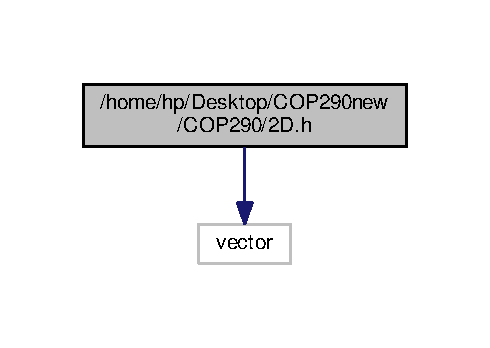
\includegraphics[width=235pt]{2_d_8h__incl}
\end{center}
\end{figure}
This graph shows which files directly or indirectly include this file\+:
\nopagebreak
\begin{figure}[H]
\begin{center}
\leavevmode
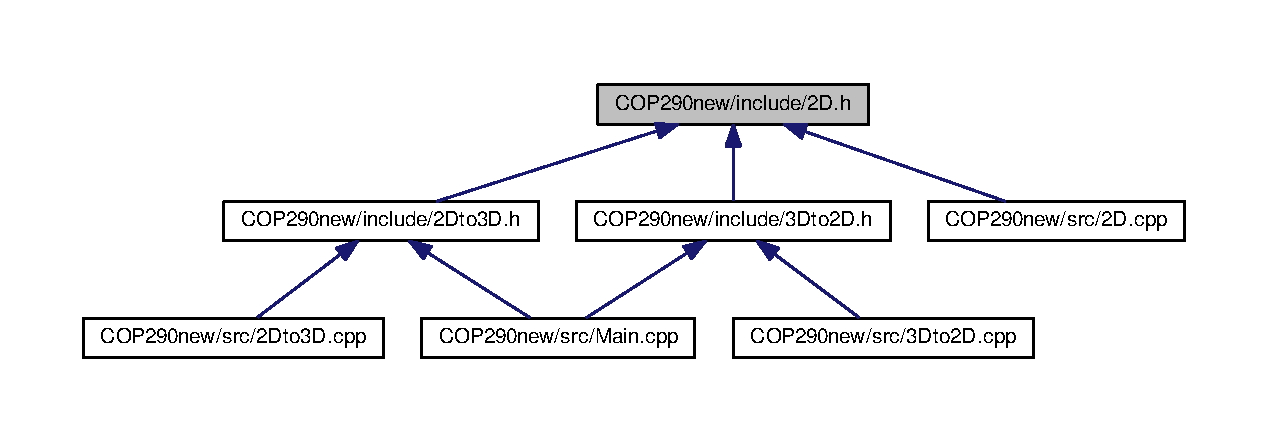
\includegraphics[width=350pt]{2_d_8h__dep__incl}
\end{center}
\end{figure}
\subsection*{Classes}
\begin{DoxyCompactItemize}
\item 
class \hyperlink{class_vertex2_d}{Vertex2D}
\item 
class \hyperlink{class_visible_edge}{Visible\+Edge}
\item 
class \hyperlink{class_orthographic_view}{Orthographic\+View}
\item 
class \hyperlink{class_hidden_edge}{Hidden\+Edge}
\item 
class \hyperlink{class_two_d_body}{Two\+D\+Body}
\end{DoxyCompactItemize}

\hypertarget{2_dto3_d_8h}{}\section{/home/hp/\+Desktop/\+C\+O\+P290/2\+Dto3D.h File Reference}
\label{2_dto3_d_8h}\index{/home/hp/\+Desktop/\+C\+O\+P290/2\+Dto3\+D.\+h@{/home/hp/\+Desktop/\+C\+O\+P290/2\+Dto3\+D.\+h}}
{\ttfamily \#include \char`\"{}3\+D.\+h\char`\"{}}\\*
{\ttfamily \#include \char`\"{}2\+D.\+h\char`\"{}}\\*
{\ttfamily \#include $<$iostream$>$}\\*
{\ttfamily \#include $<$fstream$>$}\\*
{\ttfamily \#include $<$string$>$}\\*
{\ttfamily \#include $<$vector$>$}\\*
Include dependency graph for 2\+Dto3D.h\+:
\nopagebreak
\begin{figure}[H]
\begin{center}
\leavevmode
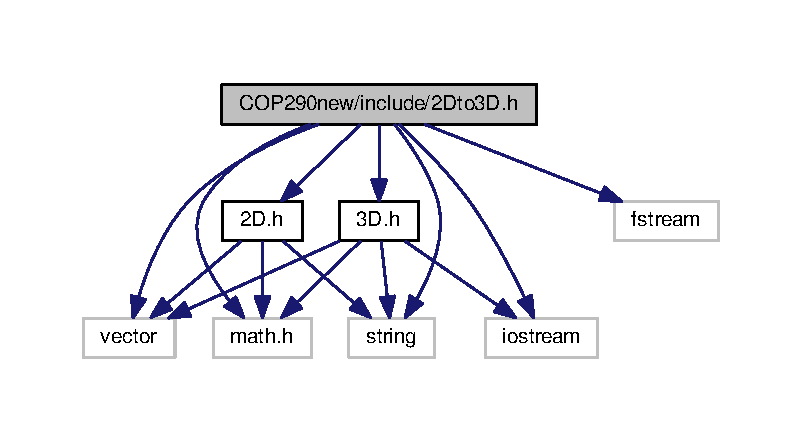
\includegraphics[width=350pt]{2_dto3_d_8h__incl}
\end{center}
\end{figure}
\subsection*{Macros}
\begin{DoxyCompactItemize}
\item 
\#define \hyperlink{2_dto3_d_8h_ac6fd404474b751c083f09311e9d421ac}{O\+D2\+\_\+H}
\end{DoxyCompactItemize}
\subsection*{Functions}
\begin{DoxyCompactItemize}
\item 
std\+::vector$<$ float $>$ \hyperlink{2_dto3_d_8h_a2075cf7d8a5a2b03b220625722bae4b3}{normalofplane} (char $\ast$plane)
\item 
void \hyperlink{2_dto3_d_8h_a776e08df14c4c59ad7d987e9cb1cd812}{viewtype} (\hyperlink{class_two_d_body}{Two\+D\+Body} twodbody)
\item 
void \hyperlink{2_dto3_d_8h_af0b2f2ff42232b5e6978d976cff35455}{topological\+Representation} (\hyperlink{class_two_d_body}{Two\+D\+Body} twodbody)
\item 
void \hyperlink{2_dto3_d_8h_a424d19e29f567e291bb3a272a2607258}{three\+D\+Reconstruct} (\hyperlink{class_two_d_body}{Two\+D\+Body} twodbody, Threebody threebody)
\end{DoxyCompactItemize}


\subsection{Macro Definition Documentation}
\index{2\+Dto3\+D.\+h@{2\+Dto3\+D.\+h}!O\+D2\+\_\+H@{O\+D2\+\_\+H}}
\index{O\+D2\+\_\+H@{O\+D2\+\_\+H}!2\+Dto3\+D.\+h@{2\+Dto3\+D.\+h}}
\subsubsection[{\texorpdfstring{O\+D2\+\_\+H}{OD2_H}}]{\setlength{\rightskip}{0pt plus 5cm}\#define O\+D2\+\_\+H}\hypertarget{2_dto3_d_8h_ac6fd404474b751c083f09311e9d421ac}{}\label{2_dto3_d_8h_ac6fd404474b751c083f09311e9d421ac}


\subsection{Function Documentation}
\index{2\+Dto3\+D.\+h@{2\+Dto3\+D.\+h}!normalofplane@{normalofplane}}
\index{normalofplane@{normalofplane}!2\+Dto3\+D.\+h@{2\+Dto3\+D.\+h}}
\subsubsection[{\texorpdfstring{normalofplane(char $\ast$plane)}{normalofplane(char *plane)}}]{\setlength{\rightskip}{0pt plus 5cm}std\+::vector$<$float$>$ normalofplane (
\begin{DoxyParamCaption}
\item[{char $\ast$}]{plane}
\end{DoxyParamCaption}
)}\hypertarget{2_dto3_d_8h_a2075cf7d8a5a2b03b220625722bae4b3}{}\label{2_dto3_d_8h_a2075cf7d8a5a2b03b220625722bae4b3}
\index{2\+Dto3\+D.\+h@{2\+Dto3\+D.\+h}!three\+D\+Reconstruct@{three\+D\+Reconstruct}}
\index{three\+D\+Reconstruct@{three\+D\+Reconstruct}!2\+Dto3\+D.\+h@{2\+Dto3\+D.\+h}}
\subsubsection[{\texorpdfstring{three\+D\+Reconstruct(\+Two\+D\+Body twodbody, Threebody threebody)}{threeDReconstruct(TwoDBody twodbody, Threebody threebody)}}]{\setlength{\rightskip}{0pt plus 5cm}void three\+D\+Reconstruct (
\begin{DoxyParamCaption}
\item[{{\bf Two\+D\+Body}}]{twodbody, }
\item[{Threebody}]{threebody}
\end{DoxyParamCaption}
)}\hypertarget{2_dto3_d_8h_a424d19e29f567e291bb3a272a2607258}{}\label{2_dto3_d_8h_a424d19e29f567e291bb3a272a2607258}
\index{2\+Dto3\+D.\+h@{2\+Dto3\+D.\+h}!topological\+Representation@{topological\+Representation}}
\index{topological\+Representation@{topological\+Representation}!2\+Dto3\+D.\+h@{2\+Dto3\+D.\+h}}
\subsubsection[{\texorpdfstring{topological\+Representation(\+Two\+D\+Body twodbody)}{topologicalRepresentation(TwoDBody twodbody)}}]{\setlength{\rightskip}{0pt plus 5cm}void topological\+Representation (
\begin{DoxyParamCaption}
\item[{{\bf Two\+D\+Body}}]{twodbody}
\end{DoxyParamCaption}
)}\hypertarget{2_dto3_d_8h_af0b2f2ff42232b5e6978d976cff35455}{}\label{2_dto3_d_8h_af0b2f2ff42232b5e6978d976cff35455}
\index{2\+Dto3\+D.\+h@{2\+Dto3\+D.\+h}!viewtype@{viewtype}}
\index{viewtype@{viewtype}!2\+Dto3\+D.\+h@{2\+Dto3\+D.\+h}}
\subsubsection[{\texorpdfstring{viewtype(\+Two\+D\+Body twodbody)}{viewtype(TwoDBody twodbody)}}]{\setlength{\rightskip}{0pt plus 5cm}void viewtype (
\begin{DoxyParamCaption}
\item[{{\bf Two\+D\+Body}}]{twodbody}
\end{DoxyParamCaption}
)}\hypertarget{2_dto3_d_8h_a776e08df14c4c59ad7d987e9cb1cd812}{}\label{2_dto3_d_8h_a776e08df14c4c59ad7d987e9cb1cd812}

\hypertarget{3_d_8h}{}\section{/home/hp/\+Desktop/\+C\+O\+P290/3D.h File Reference}
\label{3_d_8h}\index{/home/hp/\+Desktop/\+C\+O\+P290/3\+D.\+h@{/home/hp/\+Desktop/\+C\+O\+P290/3\+D.\+h}}
{\ttfamily \#include $<$vector$>$}\\*
Include dependency graph for 3D.h\+:
\nopagebreak
\begin{figure}[H]
\begin{center}
\leavevmode
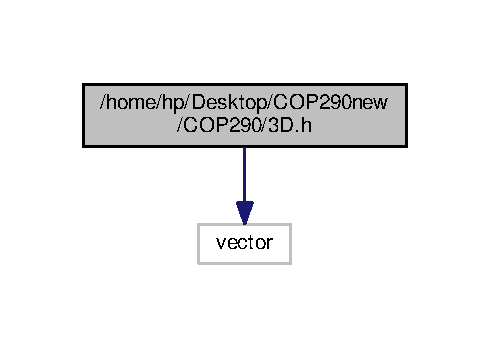
\includegraphics[width=241pt]{3_d_8h__incl}
\end{center}
\end{figure}
This graph shows which files directly or indirectly include this file\+:
\nopagebreak
\begin{figure}[H]
\begin{center}
\leavevmode
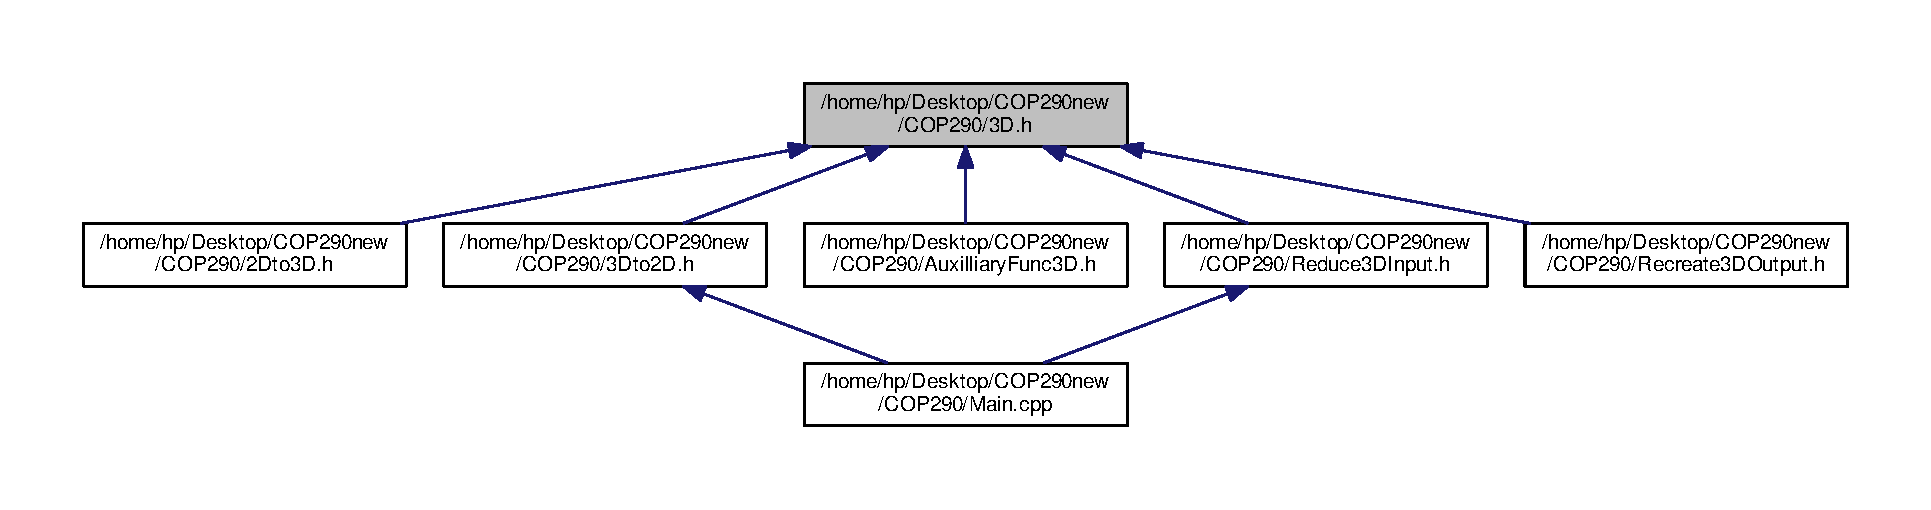
\includegraphics[width=350pt]{3_d_8h__dep__incl}
\end{center}
\end{figure}
\subsection*{Classes}
\begin{DoxyCompactItemize}
\item 
class \hyperlink{class_vertex3_d}{Vertex3D}
\item 
class \hyperlink{class_edge3_d}{Edge3D}
\item 
class \hyperlink{class_plane3_d}{Plane3D}
\item 
class \hyperlink{class_hidden_edge3_d}{Hidden\+Edge3D}
\item 
class \hyperlink{class_visible_edge3_d}{Visible\+Edge3D}
\item 
class \hyperlink{class_three_d_body}{Three\+D\+Body}
\end{DoxyCompactItemize}

\hypertarget{3_dto2_d_8h}{}\section{/home/hp/\+Desktop/\+C\+O\+P290new/\+C\+O\+P290/3\+Dto2D.h File Reference}
\label{3_dto2_d_8h}\index{/home/hp/\+Desktop/\+C\+O\+P290new/\+C\+O\+P290/3\+Dto2\+D.\+h@{/home/hp/\+Desktop/\+C\+O\+P290new/\+C\+O\+P290/3\+Dto2\+D.\+h}}
{\ttfamily \#include \char`\"{}3\+D.\+h\char`\"{}}\\*
{\ttfamily \#include \char`\"{}2\+D.\+h\char`\"{}}\\*
{\ttfamily \#include $<$iostream$>$}\\*
{\ttfamily \#include $<$fstream$>$}\\*
{\ttfamily \#include $<$string$>$}\\*
{\ttfamily \#include $<$vector$>$}\\*
Include dependency graph for 3\+Dto2D.h\+:\nopagebreak
\begin{figure}[H]
\begin{center}
\leavevmode
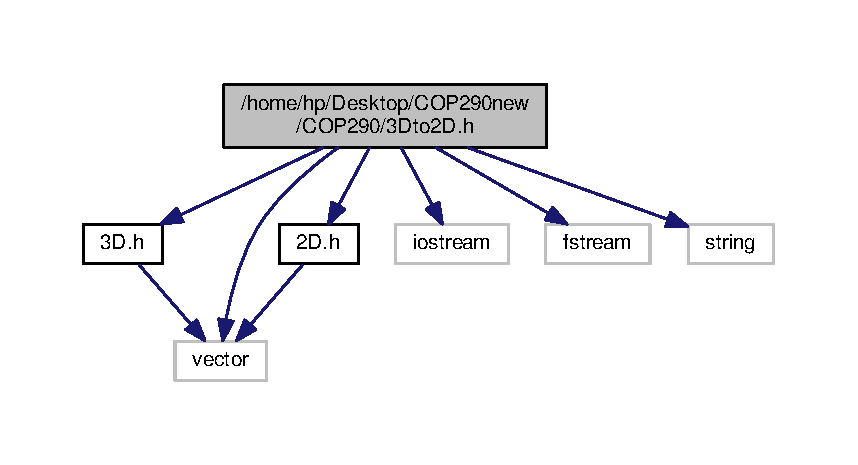
\includegraphics[width=350pt]{3_dto2_d_8h__incl}
\end{center}
\end{figure}
This graph shows which files directly or indirectly include this file\+:\nopagebreak
\begin{figure}[H]
\begin{center}
\leavevmode
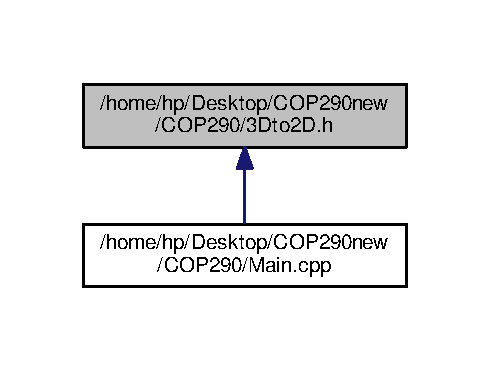
\includegraphics[width=235pt]{3_dto2_d_8h__dep__incl}
\end{center}
\end{figure}
\subsection*{Macros}
\begin{DoxyCompactItemize}
\item 
\#define \hyperlink{3_dto2_d_8h_ac6fd404474b751c083f09311e9d421ac}{O\+D2\+\_\+H}
\end{DoxyCompactItemize}
\subsection*{Functions}
\begin{DoxyCompactItemize}
\item 
std\+::vector$<$ float $>$ \hyperlink{3_dto2_d_8h_a2075cf7d8a5a2b03b220625722bae4b3}{normalofplane} (char $\ast$plane)
\item 
void \hyperlink{3_dto2_d_8h_a9e1f994f69503bda7909e8a017c17b3c}{rotate3D} (\hyperlink{class_three_d_body}{Three\+D\+Body} threedbody, std\+::vector$<$ float $>$ normal, std\+::vector$<$ char $>$ plane)
\item 
void \hyperlink{3_dto2_d_8h_a6aa5b86a823784b89de44bee6a057b7a}{hiddenedgedetection} (\hyperlink{class_three_d_body}{Three\+D\+Body} threedbody, std\+::vector$<$ char $>$ plane)
\item 
\hyperlink{class_two_d_body}{Two\+D\+Body} \hyperlink{3_dto2_d_8h_adda06f7fdd657e0b2430b637007df3a8}{Top\+View} (\hyperlink{class_three_d_body}{Three\+D\+Body} threedbody)
\end{DoxyCompactItemize}


\subsection{Macro Definition Documentation}
\index{3\+Dto2\+D.\+h@{3\+Dto2\+D.\+h}!O\+D2\+\_\+H@{O\+D2\+\_\+H}}
\index{O\+D2\+\_\+H@{O\+D2\+\_\+H}!3\+Dto2\+D.\+h@{3\+Dto2\+D.\+h}}
\subsubsection[{\texorpdfstring{O\+D2\+\_\+H}{OD2_H}}]{\setlength{\rightskip}{0pt plus 5cm}\#define O\+D2\+\_\+H}\hypertarget{3_dto2_d_8h_ac6fd404474b751c083f09311e9d421ac}{}\label{3_dto2_d_8h_ac6fd404474b751c083f09311e9d421ac}


\subsection{Function Documentation}
\index{3\+Dto2\+D.\+h@{3\+Dto2\+D.\+h}!hiddenedgedetection@{hiddenedgedetection}}
\index{hiddenedgedetection@{hiddenedgedetection}!3\+Dto2\+D.\+h@{3\+Dto2\+D.\+h}}
\subsubsection[{\texorpdfstring{hiddenedgedetection(\+Three\+D\+Body threedbody, std\+::vector$<$ char $>$ plane)}{hiddenedgedetection(ThreeDBody threedbody, std::vector< char > plane)}}]{\setlength{\rightskip}{0pt plus 5cm}void hiddenedgedetection (
\begin{DoxyParamCaption}
\item[{{\bf Three\+D\+Body}}]{threedbody, }
\item[{std\+::vector$<$ char $>$}]{plane}
\end{DoxyParamCaption}
)}\hypertarget{3_dto2_d_8h_a6aa5b86a823784b89de44bee6a057b7a}{}\label{3_dto2_d_8h_a6aa5b86a823784b89de44bee6a057b7a}
\index{3\+Dto2\+D.\+h@{3\+Dto2\+D.\+h}!normalofplane@{normalofplane}}
\index{normalofplane@{normalofplane}!3\+Dto2\+D.\+h@{3\+Dto2\+D.\+h}}
\subsubsection[{\texorpdfstring{normalofplane(char $\ast$plane)}{normalofplane(char *plane)}}]{\setlength{\rightskip}{0pt plus 5cm}std\+::vector$<$float$>$ normalofplane (
\begin{DoxyParamCaption}
\item[{char $\ast$}]{plane}
\end{DoxyParamCaption}
)}\hypertarget{3_dto2_d_8h_a2075cf7d8a5a2b03b220625722bae4b3}{}\label{3_dto2_d_8h_a2075cf7d8a5a2b03b220625722bae4b3}
\index{3\+Dto2\+D.\+h@{3\+Dto2\+D.\+h}!rotate3D@{rotate3D}}
\index{rotate3D@{rotate3D}!3\+Dto2\+D.\+h@{3\+Dto2\+D.\+h}}
\subsubsection[{\texorpdfstring{rotate3\+D(\+Three\+D\+Body threedbody, std\+::vector$<$ float $>$ normal, std\+::vector$<$ char $>$ plane)}{rotate3D(ThreeDBody threedbody, std::vector< float > normal, std::vector< char > plane)}}]{\setlength{\rightskip}{0pt plus 5cm}void rotate3D (
\begin{DoxyParamCaption}
\item[{{\bf Three\+D\+Body}}]{threedbody, }
\item[{std\+::vector$<$ float $>$}]{normal, }
\item[{std\+::vector$<$ char $>$}]{plane}
\end{DoxyParamCaption}
)}\hypertarget{3_dto2_d_8h_a9e1f994f69503bda7909e8a017c17b3c}{}\label{3_dto2_d_8h_a9e1f994f69503bda7909e8a017c17b3c}
\index{3\+Dto2\+D.\+h@{3\+Dto2\+D.\+h}!Top\+View@{Top\+View}}
\index{Top\+View@{Top\+View}!3\+Dto2\+D.\+h@{3\+Dto2\+D.\+h}}
\subsubsection[{\texorpdfstring{Top\+View(\+Three\+D\+Body threedbody)}{TopView(ThreeDBody threedbody)}}]{\setlength{\rightskip}{0pt plus 5cm}{\bf Two\+D\+Body} Top\+View (
\begin{DoxyParamCaption}
\item[{{\bf Three\+D\+Body}}]{threedbody}
\end{DoxyParamCaption}
)}\hypertarget{3_dto2_d_8h_adda06f7fdd657e0b2430b637007df3a8}{}\label{3_dto2_d_8h_adda06f7fdd657e0b2430b637007df3a8}

\hypertarget{myarea_8h}{}\section{C\+O\+P290new/include/myarea.h File Reference}
\label{myarea_8h}\index{C\+O\+P290new/include/myarea.\+h@{C\+O\+P290new/include/myarea.\+h}}
{\ttfamily \#include $<$gtkmm.\+h$>$}\\*
Include dependency graph for myarea.\+h\+:
\nopagebreak
\begin{figure}[H]
\begin{center}
\leavevmode
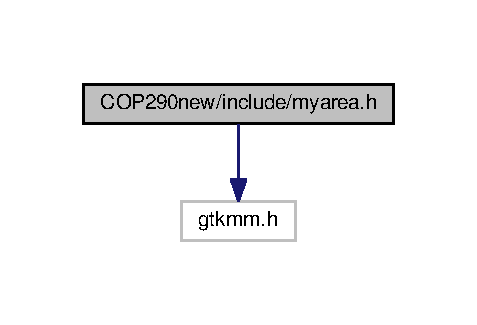
\includegraphics[width=229pt]{myarea_8h__incl}
\end{center}
\end{figure}
This graph shows which files directly or indirectly include this file\+:
\nopagebreak
\begin{figure}[H]
\begin{center}
\leavevmode
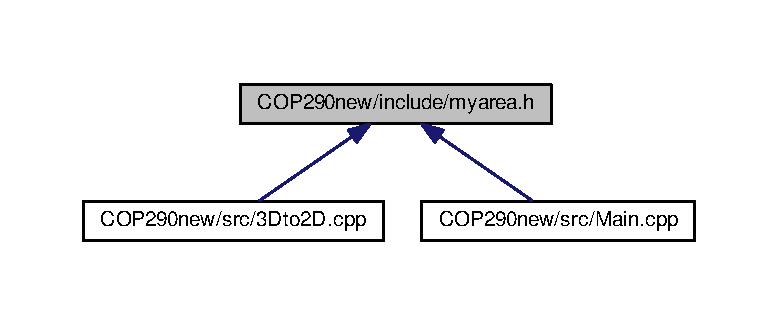
\includegraphics[width=350pt]{myarea_8h__dep__incl}
\end{center}
\end{figure}
\subsection*{Classes}
\begin{DoxyCompactItemize}
\item 
class \hyperlink{class_my_window}{My\+Window}
\item 
class \hyperlink{class_file_window}{File\+Window}
\end{DoxyCompactItemize}

\hypertarget{_readme_8md}{}\section{C\+O\+P290new/\+Readme.md File Reference}
\label{_readme_8md}\index{C\+O\+P290new/\+Readme.\+md@{C\+O\+P290new/\+Readme.\+md}}

\hypertarget{2_d_8cpp}{}\section{/home/hp/\+Desktop/\+C\+O\+P290/2D.cpp File Reference}
\label{2_d_8cpp}\index{/home/hp/\+Desktop/\+C\+O\+P290/2\+D.\+cpp@{/home/hp/\+Desktop/\+C\+O\+P290/2\+D.\+cpp}}
This graph shows which files directly or indirectly include this file\+:\nopagebreak
\begin{figure}[H]
\begin{center}
\leavevmode
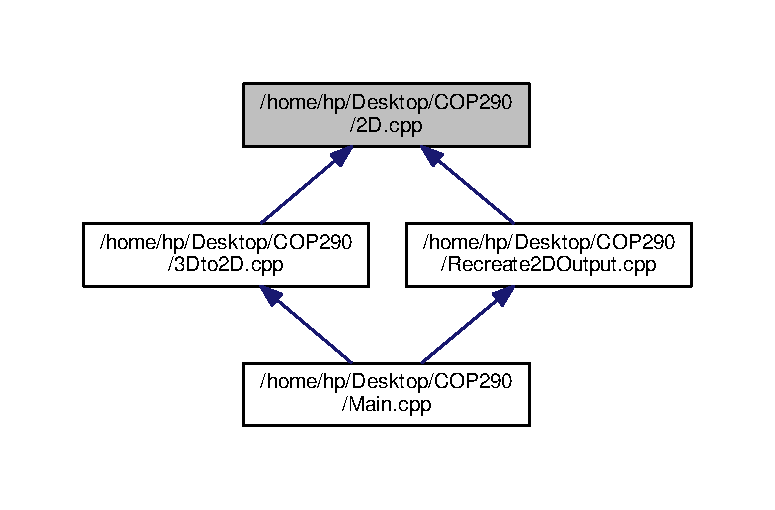
\includegraphics[width=350pt]{2_d_8cpp__dep__incl}
\end{center}
\end{figure}
\subsection*{Classes}
\begin{DoxyCompactItemize}
\item 
class \hyperlink{class_vertex2_d}{Vertex2D}
\item 
class \hyperlink{class_visible_edge}{Visible\+Edge}
\item 
class \hyperlink{class_hidden_edge}{Hidden\+Edge}
\item 
class \hyperlink{class_two_d_body}{Two\+D\+Body}
\end{DoxyCompactItemize}

\hypertarget{2_dto3_d_8cpp}{}\section{C\+O\+P290new/src/2\+Dto3D.cpp File Reference}
\label{2_dto3_d_8cpp}\index{C\+O\+P290new/src/2\+Dto3\+D.\+cpp@{C\+O\+P290new/src/2\+Dto3\+D.\+cpp}}
{\ttfamily \#include \char`\"{}2\+Dto3\+D.\+h\char`\"{}}\\*
Include dependency graph for 2\+Dto3D.cpp\+:
\nopagebreak
\begin{figure}[H]
\begin{center}
\leavevmode
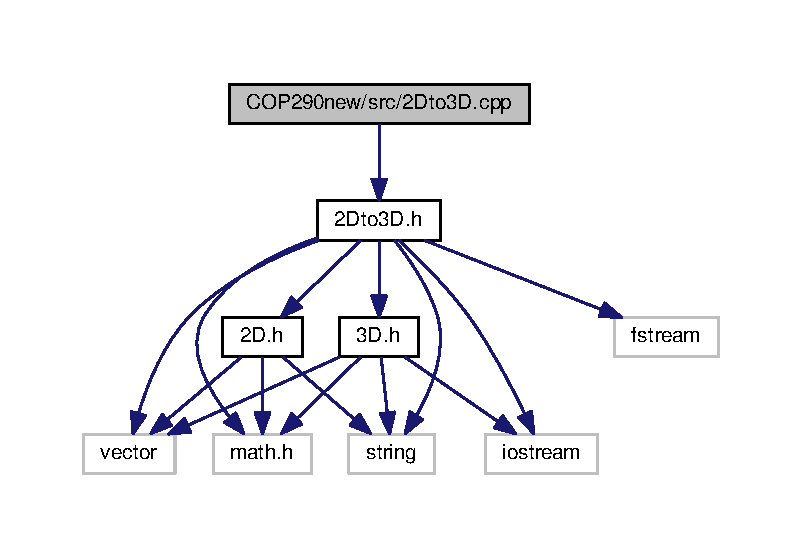
\includegraphics[width=350pt]{2_dto3_d_8cpp__incl}
\end{center}
\end{figure}
\subsection*{Functions}
\begin{DoxyCompactItemize}
\item 
\hyperlink{class_three_d_body}{Three\+D\+Body} \hyperlink{2_dto3_d_8cpp_a8e5645af1925f57d823b1975286d007e}{three\+Dlabel} (\hyperlink{class_two_d_body}{Two\+D\+Body} \&top, \hyperlink{class_two_d_body}{Two\+D\+Body} \&front, \hyperlink{class_two_d_body}{Two\+D\+Body} \&left)
\end{DoxyCompactItemize}


\subsection{Function Documentation}
\index{2\+Dto3\+D.\+cpp@{2\+Dto3\+D.\+cpp}!three\+Dlabel@{three\+Dlabel}}
\index{three\+Dlabel@{three\+Dlabel}!2\+Dto3\+D.\+cpp@{2\+Dto3\+D.\+cpp}}
\subsubsection[{\texorpdfstring{three\+Dlabel(\+Two\+D\+Body \&top, Two\+D\+Body \&front, Two\+D\+Body \&left)}{threeDlabel(TwoDBody &top, TwoDBody &front, TwoDBody &left)}}]{\setlength{\rightskip}{0pt plus 5cm}{\bf Three\+D\+Body} three\+Dlabel (
\begin{DoxyParamCaption}
\item[{{\bf Two\+D\+Body} \&}]{top, }
\item[{{\bf Two\+D\+Body} \&}]{front, }
\item[{{\bf Two\+D\+Body} \&}]{left}
\end{DoxyParamCaption}
)}\hypertarget{2_dto3_d_8cpp_a8e5645af1925f57d823b1975286d007e}{}\label{2_dto3_d_8cpp_a8e5645af1925f57d823b1975286d007e}

\hypertarget{3_d_8cpp}{}\section{/home/hp/\+Desktop/\+C\+O\+P290/3D.cpp File Reference}
\label{3_d_8cpp}\index{/home/hp/\+Desktop/\+C\+O\+P290/3\+D.\+cpp@{/home/hp/\+Desktop/\+C\+O\+P290/3\+D.\+cpp}}
This graph shows which files directly or indirectly include this file\+:\nopagebreak
\begin{figure}[H]
\begin{center}
\leavevmode
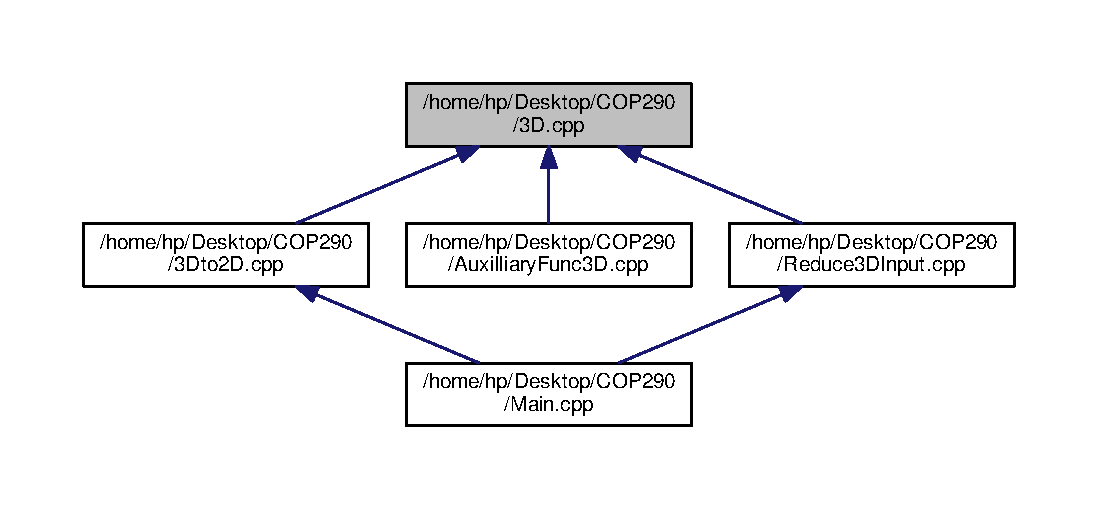
\includegraphics[width=350pt]{3_d_8cpp__dep__incl}
\end{center}
\end{figure}
\subsection*{Classes}
\begin{DoxyCompactItemize}
\item 
class \hyperlink{class_vertex3_d}{Vertex3D}
\item 
class \hyperlink{class_edge3_d}{Edge3D}
\item 
class \hyperlink{class_plane3_d}{Plane3D}
\item 
class \hyperlink{class_hidden_edge3_d}{Hidden\+Edge3D}
\item 
class \hyperlink{class_visible_edge3_d}{Visible\+Edge3D}
\item 
class \hyperlink{class_three_d_body}{Three\+D\+Body}
\end{DoxyCompactItemize}

\hypertarget{3_dto2_d_8cpp}{}\section{C\+O\+P290new/src/3\+Dto2D.cpp File Reference}
\label{3_dto2_d_8cpp}\index{C\+O\+P290new/src/3\+Dto2\+D.\+cpp@{C\+O\+P290new/src/3\+Dto2\+D.\+cpp}}
{\ttfamily \#include \char`\"{}3\+Dto2\+D.\+h\char`\"{}}\\*
{\ttfamily \#include \char`\"{}myarea.\+h\char`\"{}}\\*
{\ttfamily \#include $<$cairomm/context.\+h$>$}\\*
Include dependency graph for 3\+Dto2D.cpp\+:
\nopagebreak
\begin{figure}[H]
\begin{center}
\leavevmode
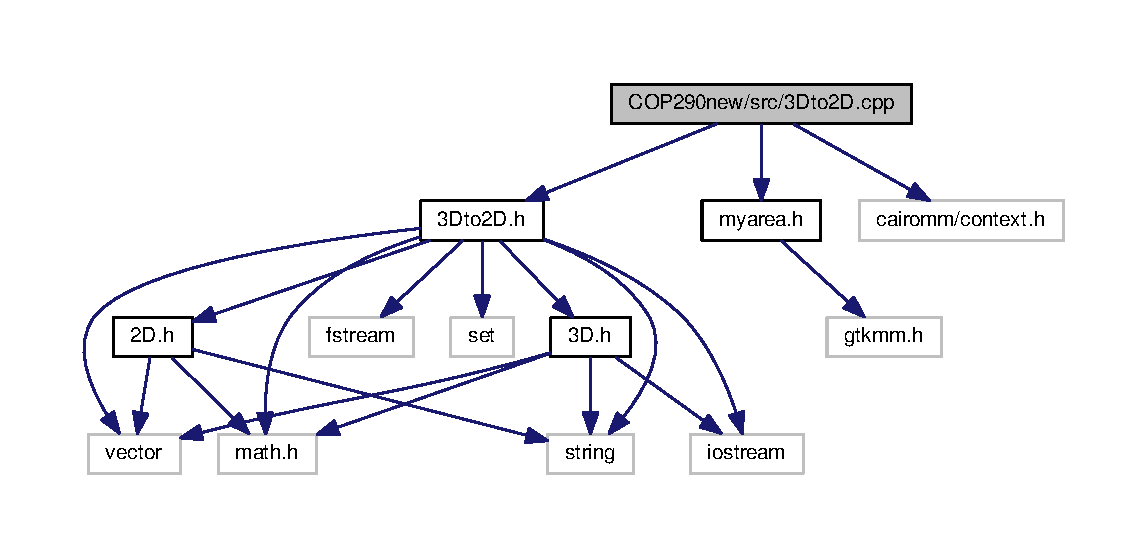
\includegraphics[width=350pt]{3_dto2_d_8cpp__incl}
\end{center}
\end{figure}
\subsection*{Functions}
\begin{DoxyCompactItemize}
\item 
std\+::vector$<$ double $>$ \hyperlink{3_dto2_d_8cpp_aa1d5affc106c07f4e11f26ef6ce62499}{normalofplane} (double a, double b, double c, double d)
\item 
\hyperlink{class_three_d_body}{Three\+D\+Body} \hyperlink{3_dto2_d_8cpp_a863c474ca58c668c1b2be377198e8241}{rotate3D} (\hyperlink{class_three_d_body}{Three\+D\+Body} \&threedbody, std\+::vector$<$ double $>$ normal)
\item 
std\+::vector$<$ \hyperlink{class_edge3_d}{Edge3D} $>$ \hyperlink{3_dto2_d_8cpp_aaf0349dc7b34ca0c038b764c2be18aec}{edge\+\_\+segmentation} (\hyperlink{class_three_d_body}{Three\+D\+Body} \&threedbody)
\item 
void \hyperlink{3_dto2_d_8cpp_a300480e6d73c1684365a6ab0755f9f29}{cross\+Product} (double vect\+\_\+A\mbox{[}$\,$\mbox{]}, double vect\+\_\+B\mbox{[}$\,$\mbox{]}, double cross\+\_\+P\mbox{[}$\,$\mbox{]})
\item 
int \hyperlink{3_dto2_d_8cpp_a8a2c17d457d67148ccf5b95d2b18dcce}{raycast} (double x, double y, \hyperlink{class_plane2_d}{Plane2D} plane)
\item 
void \hyperlink{3_dto2_d_8cpp_aac1981fc6e5c4b2b9656cc816f2cb1d4}{hiddenedgedetection} (\hyperlink{class_three_d_body}{Three\+D\+Body} \&threedbody, double a, double b, double c, double d)
\item 
\hyperlink{class_two_d_body}{Two\+D\+Body} \hyperlink{3_dto2_d_8cpp_a467808619d4c582f765b502afac56599}{Top\+View} (\hyperlink{class_three_d_body}{Three\+D\+Body} \&threedbody)
\item 
void \hyperlink{3_dto2_d_8cpp_a28ad79f36a5e3dde8f6c201df6301af1}{Three\+D\+Bodi} (\hyperlink{class_three_d_body}{Three\+D\+Body} need)
\item 
void \hyperlink{3_dto2_d_8cpp_a6dc63695e5e947a0258fce994e65394a}{type\+\_\+equal} (int \hyperlink{_main_8cpp_ac765329451135abec74c45e1897abf26}{type})
\end{DoxyCompactItemize}
\subsection*{Variables}
\begin{DoxyCompactItemize}
\item 
int \hyperlink{3_dto2_d_8cpp_a32b56170ed65ed9c964cd7c674a2f3de}{type1}
\item 
\hyperlink{class_two_d_body}{Two\+D\+Body} \hyperlink{3_dto2_d_8cpp_abb3a0338db8b77077ff59ad43fd7a473}{twodbodyy}
\item 
\hyperlink{class_three_d_body}{Three\+D\+Body} \hyperlink{3_dto2_d_8cpp_a70dd0000c56b8437e1010643c626ee10}{wire\+\_\+frame}
\end{DoxyCompactItemize}


\subsection{Function Documentation}
\index{3\+Dto2\+D.\+cpp@{3\+Dto2\+D.\+cpp}!cross\+Product@{cross\+Product}}
\index{cross\+Product@{cross\+Product}!3\+Dto2\+D.\+cpp@{3\+Dto2\+D.\+cpp}}
\subsubsection[{\texorpdfstring{cross\+Product(double vect\+\_\+A[], double vect\+\_\+B[], double cross\+\_\+P[])}{crossProduct(double vect_A[], double vect_B[], double cross_P[])}}]{\setlength{\rightskip}{0pt plus 5cm}void cross\+Product (
\begin{DoxyParamCaption}
\item[{double}]{vect\+\_\+A\mbox{[}$\,$\mbox{]}, }
\item[{double}]{vect\+\_\+B\mbox{[}$\,$\mbox{]}, }
\item[{double}]{cross\+\_\+P\mbox{[}$\,$\mbox{]}}
\end{DoxyParamCaption}
)}\hypertarget{3_dto2_d_8cpp_a300480e6d73c1684365a6ab0755f9f29}{}\label{3_dto2_d_8cpp_a300480e6d73c1684365a6ab0755f9f29}
\index{3\+Dto2\+D.\+cpp@{3\+Dto2\+D.\+cpp}!edge\+\_\+segmentation@{edge\+\_\+segmentation}}
\index{edge\+\_\+segmentation@{edge\+\_\+segmentation}!3\+Dto2\+D.\+cpp@{3\+Dto2\+D.\+cpp}}
\subsubsection[{\texorpdfstring{edge\+\_\+segmentation(\+Three\+D\+Body \&threedbody)}{edge_segmentation(ThreeDBody &threedbody)}}]{\setlength{\rightskip}{0pt plus 5cm}std\+::vector$<${\bf Edge3D}$>$ edge\+\_\+segmentation (
\begin{DoxyParamCaption}
\item[{{\bf Three\+D\+Body} \&}]{threedbody}
\end{DoxyParamCaption}
)}\hypertarget{3_dto2_d_8cpp_aaf0349dc7b34ca0c038b764c2be18aec}{}\label{3_dto2_d_8cpp_aaf0349dc7b34ca0c038b764c2be18aec}
\index{3\+Dto2\+D.\+cpp@{3\+Dto2\+D.\+cpp}!hiddenedgedetection@{hiddenedgedetection}}
\index{hiddenedgedetection@{hiddenedgedetection}!3\+Dto2\+D.\+cpp@{3\+Dto2\+D.\+cpp}}
\subsubsection[{\texorpdfstring{hiddenedgedetection(\+Three\+D\+Body \&threedbody, double a, double b, double c, double d)}{hiddenedgedetection(ThreeDBody &threedbody, double a, double b, double c, double d)}}]{\setlength{\rightskip}{0pt plus 5cm}void hiddenedgedetection (
\begin{DoxyParamCaption}
\item[{{\bf Three\+D\+Body} \&}]{threedbody, }
\item[{double}]{a, }
\item[{double}]{b, }
\item[{double}]{c, }
\item[{double}]{d}
\end{DoxyParamCaption}
)}\hypertarget{3_dto2_d_8cpp_aac1981fc6e5c4b2b9656cc816f2cb1d4}{}\label{3_dto2_d_8cpp_aac1981fc6e5c4b2b9656cc816f2cb1d4}


Here is the call graph for this function\+:
\nopagebreak
\begin{figure}[H]
\begin{center}
\leavevmode
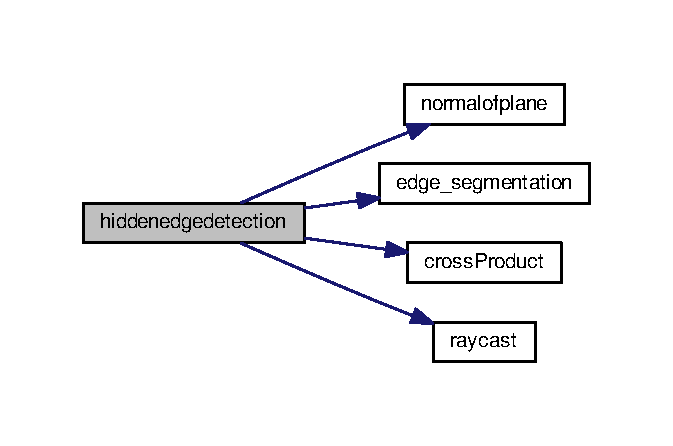
\includegraphics[width=323pt]{3_dto2_d_8cpp_aac1981fc6e5c4b2b9656cc816f2cb1d4_cgraph}
\end{center}
\end{figure}


\index{3\+Dto2\+D.\+cpp@{3\+Dto2\+D.\+cpp}!normalofplane@{normalofplane}}
\index{normalofplane@{normalofplane}!3\+Dto2\+D.\+cpp@{3\+Dto2\+D.\+cpp}}
\subsubsection[{\texorpdfstring{normalofplane(double a, double b, double c, double d)}{normalofplane(double a, double b, double c, double d)}}]{\setlength{\rightskip}{0pt plus 5cm}std\+::vector$<$double$>$ normalofplane (
\begin{DoxyParamCaption}
\item[{double}]{a, }
\item[{double}]{b, }
\item[{double}]{c, }
\item[{double}]{d}
\end{DoxyParamCaption}
)}\hypertarget{3_dto2_d_8cpp_aa1d5affc106c07f4e11f26ef6ce62499}{}\label{3_dto2_d_8cpp_aa1d5affc106c07f4e11f26ef6ce62499}
\index{3\+Dto2\+D.\+cpp@{3\+Dto2\+D.\+cpp}!raycast@{raycast}}
\index{raycast@{raycast}!3\+Dto2\+D.\+cpp@{3\+Dto2\+D.\+cpp}}
\subsubsection[{\texorpdfstring{raycast(double x, double y, Plane2\+D plane)}{raycast(double x, double y, Plane2D plane)}}]{\setlength{\rightskip}{0pt plus 5cm}int raycast (
\begin{DoxyParamCaption}
\item[{double}]{x, }
\item[{double}]{y, }
\item[{{\bf Plane2D}}]{plane}
\end{DoxyParamCaption}
)}\hypertarget{3_dto2_d_8cpp_a8a2c17d457d67148ccf5b95d2b18dcce}{}\label{3_dto2_d_8cpp_a8a2c17d457d67148ccf5b95d2b18dcce}
\index{3\+Dto2\+D.\+cpp@{3\+Dto2\+D.\+cpp}!rotate3D@{rotate3D}}
\index{rotate3D@{rotate3D}!3\+Dto2\+D.\+cpp@{3\+Dto2\+D.\+cpp}}
\subsubsection[{\texorpdfstring{rotate3\+D(\+Three\+D\+Body \&threedbody, std\+::vector$<$ double $>$ normal)}{rotate3D(ThreeDBody &threedbody, std::vector< double > normal)}}]{\setlength{\rightskip}{0pt plus 5cm}{\bf Three\+D\+Body} rotate3D (
\begin{DoxyParamCaption}
\item[{{\bf Three\+D\+Body} \&}]{threedbody, }
\item[{std\+::vector$<$ double $>$}]{normal}
\end{DoxyParamCaption}
)}\hypertarget{3_dto2_d_8cpp_a863c474ca58c668c1b2be377198e8241}{}\label{3_dto2_d_8cpp_a863c474ca58c668c1b2be377198e8241}
\index{3\+Dto2\+D.\+cpp@{3\+Dto2\+D.\+cpp}!Three\+D\+Bodi@{Three\+D\+Bodi}}
\index{Three\+D\+Bodi@{Three\+D\+Bodi}!3\+Dto2\+D.\+cpp@{3\+Dto2\+D.\+cpp}}
\subsubsection[{\texorpdfstring{Three\+D\+Bodi(\+Three\+D\+Body need)}{ThreeDBodi(ThreeDBody need)}}]{\setlength{\rightskip}{0pt plus 5cm}void Three\+D\+Bodi (
\begin{DoxyParamCaption}
\item[{{\bf Three\+D\+Body}}]{need}
\end{DoxyParamCaption}
)}\hypertarget{3_dto2_d_8cpp_a28ad79f36a5e3dde8f6c201df6301af1}{}\label{3_dto2_d_8cpp_a28ad79f36a5e3dde8f6c201df6301af1}
\index{3\+Dto2\+D.\+cpp@{3\+Dto2\+D.\+cpp}!Top\+View@{Top\+View}}
\index{Top\+View@{Top\+View}!3\+Dto2\+D.\+cpp@{3\+Dto2\+D.\+cpp}}
\subsubsection[{\texorpdfstring{Top\+View(\+Three\+D\+Body \&threedbody)}{TopView(ThreeDBody &threedbody)}}]{\setlength{\rightskip}{0pt plus 5cm}{\bf Two\+D\+Body} Top\+View (
\begin{DoxyParamCaption}
\item[{{\bf Three\+D\+Body} \&}]{threedbody}
\end{DoxyParamCaption}
)}\hypertarget{3_dto2_d_8cpp_a467808619d4c582f765b502afac56599}{}\label{3_dto2_d_8cpp_a467808619d4c582f765b502afac56599}
\index{3\+Dto2\+D.\+cpp@{3\+Dto2\+D.\+cpp}!type\+\_\+equal@{type\+\_\+equal}}
\index{type\+\_\+equal@{type\+\_\+equal}!3\+Dto2\+D.\+cpp@{3\+Dto2\+D.\+cpp}}
\subsubsection[{\texorpdfstring{type\+\_\+equal(int type)}{type_equal(int type)}}]{\setlength{\rightskip}{0pt plus 5cm}void type\+\_\+equal (
\begin{DoxyParamCaption}
\item[{int}]{type}
\end{DoxyParamCaption}
)}\hypertarget{3_dto2_d_8cpp_a6dc63695e5e947a0258fce994e65394a}{}\label{3_dto2_d_8cpp_a6dc63695e5e947a0258fce994e65394a}


\subsection{Variable Documentation}
\index{3\+Dto2\+D.\+cpp@{3\+Dto2\+D.\+cpp}!twodbodyy@{twodbodyy}}
\index{twodbodyy@{twodbodyy}!3\+Dto2\+D.\+cpp@{3\+Dto2\+D.\+cpp}}
\subsubsection[{\texorpdfstring{twodbodyy}{twodbodyy}}]{\setlength{\rightskip}{0pt plus 5cm}{\bf Two\+D\+Body} twodbodyy}\hypertarget{3_dto2_d_8cpp_abb3a0338db8b77077ff59ad43fd7a473}{}\label{3_dto2_d_8cpp_abb3a0338db8b77077ff59ad43fd7a473}
\index{3\+Dto2\+D.\+cpp@{3\+Dto2\+D.\+cpp}!type1@{type1}}
\index{type1@{type1}!3\+Dto2\+D.\+cpp@{3\+Dto2\+D.\+cpp}}
\subsubsection[{\texorpdfstring{type1}{type1}}]{\setlength{\rightskip}{0pt plus 5cm}int type1}\hypertarget{3_dto2_d_8cpp_a32b56170ed65ed9c964cd7c674a2f3de}{}\label{3_dto2_d_8cpp_a32b56170ed65ed9c964cd7c674a2f3de}
\index{3\+Dto2\+D.\+cpp@{3\+Dto2\+D.\+cpp}!wire\+\_\+frame@{wire\+\_\+frame}}
\index{wire\+\_\+frame@{wire\+\_\+frame}!3\+Dto2\+D.\+cpp@{3\+Dto2\+D.\+cpp}}
\subsubsection[{\texorpdfstring{wire\+\_\+frame}{wire_frame}}]{\setlength{\rightskip}{0pt plus 5cm}{\bf Three\+D\+Body} wire\+\_\+frame}\hypertarget{3_dto2_d_8cpp_a70dd0000c56b8437e1010643c626ee10}{}\label{3_dto2_d_8cpp_a70dd0000c56b8437e1010643c626ee10}

\hypertarget{_main_8cpp}{}\section{/home/hp/\+Desktop/\+C\+O\+P290/\+Main.cpp File Reference}
\label{_main_8cpp}\index{/home/hp/\+Desktop/\+C\+O\+P290/\+Main.\+cpp@{/home/hp/\+Desktop/\+C\+O\+P290/\+Main.\+cpp}}
{\ttfamily \#include \char`\"{}Reduce3\+D\+Input.\+h\char`\"{}}\\*
{\ttfamily \#include \char`\"{}3\+Dto2\+D.\+h\char`\"{}}\\*
{\ttfamily \#include \char`\"{}Recreate2\+D\+Output.\+h\char`\"{}}\\*
Include dependency graph for Main.\+cpp\+:
\nopagebreak
\begin{figure}[H]
\begin{center}
\leavevmode
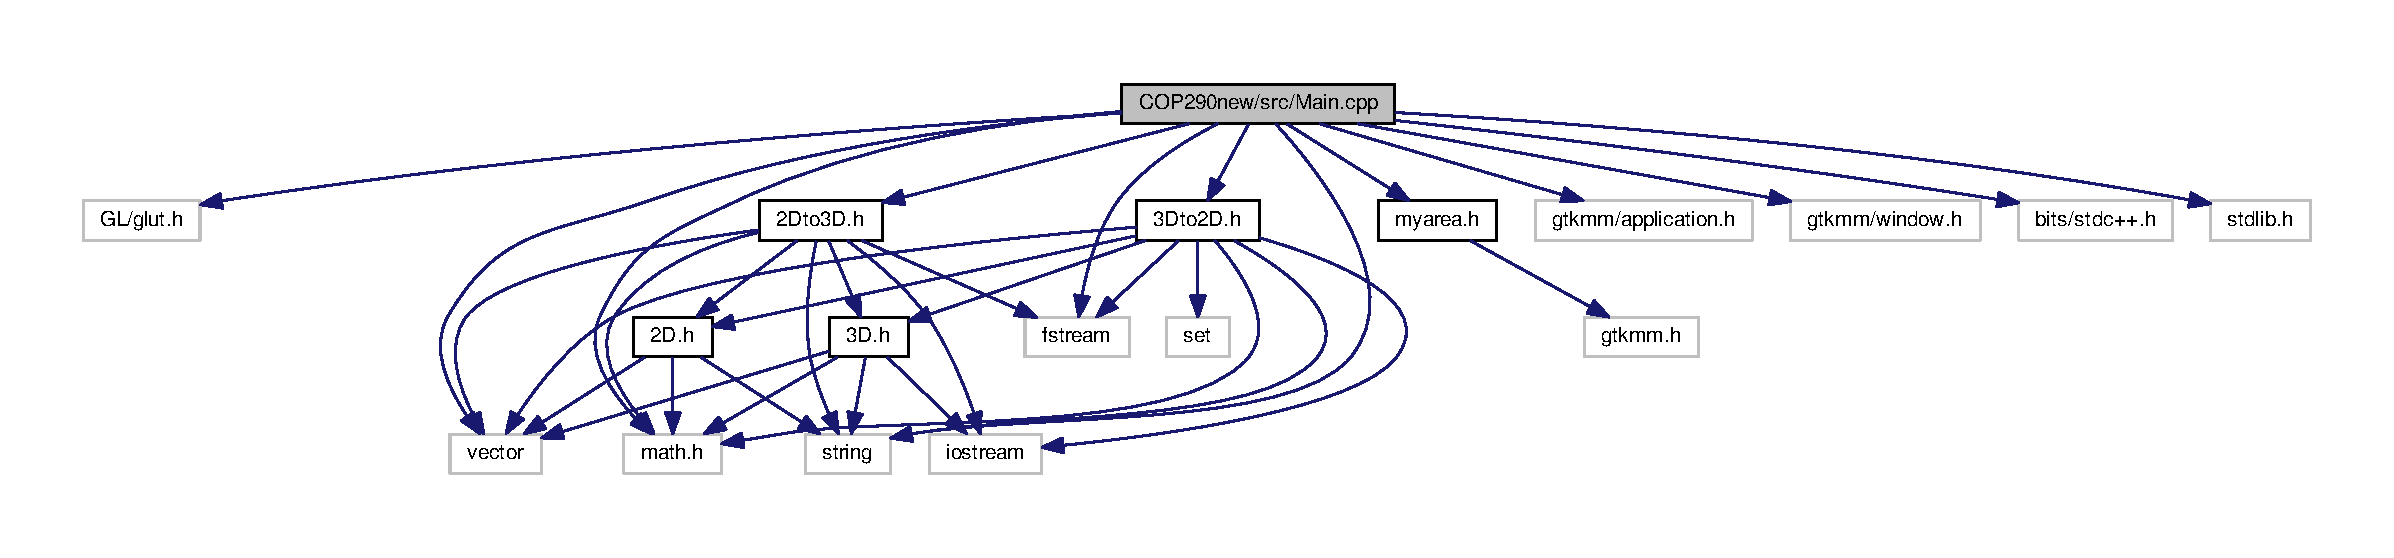
\includegraphics[width=350pt]{_main_8cpp__incl}
\end{center}
\end{figure}
\subsection*{Functions}
\begin{DoxyCompactItemize}
\item 
void \hyperlink{_main_8cpp_a0680a922e25d3366b6ab7396aabe4a49}{Three\+Dto\+TwoD} (std\+::ifstream \&Input\+File)
\end{DoxyCompactItemize}


\subsection{Function Documentation}
\index{Main.\+cpp@{Main.\+cpp}!Three\+Dto\+TwoD@{Three\+Dto\+TwoD}}
\index{Three\+Dto\+TwoD@{Three\+Dto\+TwoD}!Main.\+cpp@{Main.\+cpp}}
\subsubsection[{\texorpdfstring{Three\+Dto\+Two\+D(std\+::ifstream \&\+Input\+File)}{ThreeDtoTwoD(std::ifstream &InputFile)}}]{\setlength{\rightskip}{0pt plus 5cm}void Three\+Dto\+TwoD (
\begin{DoxyParamCaption}
\item[{std\+::ifstream \&}]{Input\+File}
\end{DoxyParamCaption}
)}\hypertarget{_main_8cpp_a0680a922e25d3366b6ab7396aabe4a49}{}\label{_main_8cpp_a0680a922e25d3366b6ab7396aabe4a49}

%--- End generated contents ---

% Index
\backmatter
\newpage
\phantomsection
\clearemptydoublepage
\addcontentsline{toc}{chapter}{Index}
\printindex

\end{document}
